\documentclass[conference]{IEEEtran}

\usepackage[T1]{fontenc}
\usepackage[utf8]{inputenc}
\usepackage{microtype}
\usepackage{booktabs}
\usepackage{array}
\usepackage{graphicx}
\usepackage{flafter}
\usepackage{float}
\usepackage{cite}
\usepackage{url}
\usepackage[hidelinks]{hyperref}
\usepackage{tikz}
\usetikzlibrary{arrows.meta,positioning,shapes.geometric,calc}

\newcommand{\system}{\textsc{Cognalys}}
\newcommand{\researchq}[1]{\textbf{RQ#1}}
\newcommand{\pending}[1]{\textbf{[TODO: #1]}}

\title{Cognalys: A Python Library Complementing RVSec with Evidence-Guided Analysis and Repair}

\author{\IEEEauthorblockN{João Pedro Antonow}
\IEEEauthorblockA{Department of Computer Science (CIC)\\
University of Brasília (UnB)\\
Brasília, Brazil\\
\texttt{jpantonow@gmail.com}\\[3pt]
Advisor: Prof.\ Rodrigo Bonifácio\\Co-advisor: Prof.\ Guilherme Novaes Ramos}}

\begin{document}

\maketitle

\begin{abstract}
RVSec reports cryptographic API misuses that an Android application executed,
but not which source change is safe: a fix can depend on stored data, protocol
peers, callers, and application policy. \system, a Python library and
command-line tool, treats each RVSec finding as a claim to check before
repairing it. With repository evidence from the analyzed revision, large
language model stages under deterministic checks decide whether the violation
is real and whether a fix keeps the application's behavior. A confirmed
violation with such a fix, even a rule-only one, becomes a patch applied in an
isolated worktree at the tip of the target branch and built; other findings
end with their reason recorded, or with an issue when their security impact
was confirmed. Nothing is published without explicit human approval.
We report a dated case study of an earlier pipeline version and two
pre-registered evaluations with declared deviations; all results are
descriptive. As of November 18, 2026, of 49 pull requests submitted for RVSec
findings from the RVSec group's campaign (8), from earlier RVSec reports (15),
and from our own RVSec runs (26), 21 were incorporated (one only adds a test), 10 were closed, and 18
were open; six of the ten closures questioned the security relevance of the
reported use. When RVSec was rerun on the original and the patched APK, the
reported violation no longer appeared in the patched method for 33 of
the 38 pull requests it could check (25 under the registered rule), and one corrected patch kept
the same key material and only changed how the monitor saw it. On 20 analysis units, two LLM judges, not told which arm produced each delivery,
compared \system{} with coding agents in two blocks. Agents given only the
finding and the repository proposed fewer pull requests than \system{}, with
fewer judged acceptable (7 to 18, against 28). Agents instructed to follow the
same process proposed more, with as many or more judged acceptable under the full
reading (28 and 32) but also more judged unacceptable (10 and 14, against 3).
A per-run score that counts issues and no-action outcomes as acceptable, and so
rewards abstention, placed the first block close to or above \system{} (0.90 to
0.97, against 0.96) and the second below it (0.85 and 0.80). Neither the build nor the rerun shows that a patch preserves the
application's behavior.
\end{abstract}

\begin{IEEEkeywords}
cryptographic API misuse, runtime verification, Android, large language
models, program repair, coding agents, open-source contributions, false
positives
\end{IEEEkeywords}

\section{Introduction}
\label{sec:introduction}

Developers struggle to use Java cryptographic APIs
correctly~\cite{nadi2016hoops}, and misuses remain common in Android
applications~\cite{egele2013crypto,costa2026rv4android}; many tools detect
them: static analyzers such as CogniCrypt and CryptoGuard, and dynamic tools
such as CryLogger and RVSec~\cite{krueger2017cognicrypt,krueger2021crysl,
rahaman2019cryptoguard,piccolboni2021crylogger,torres2023runtime}. Detection has
been studied extensively; acting on a report much less. A report says that a
rule was violated, not whether the violation matters in that application or how
to change the program without breaking it. Replacing \texttt{SHA-1} with
\texttt{SHA-256} changes the bytes that storage, synchronization, or a server
expect, and pinning a TLS version removes protocols a peer may still need. The
maintainers who answered our pull requests raised exactly these concerns:
behavior they consider intentional, the compatibility of stored values, and
whether the rule matters in their context (Section~\ref{sec:results}).

RVSec~\cite{torres2023runtime,costa2026rv4android} monitors cryptographic API calls while an
instrumented APK runs and reports each violation at the method that made the
call. Its findings show that the misuse executes, which a static warning does
not, but they refer to a compiled APK rather than to source code: the reported
method may be a Kotlin lambda or coroutine, a name changed by the compiler, or
library code bundled in the app. Turning such a finding into a change a
maintainer can accept takes three further steps: locating the code in the
repository revision the APK was built from, deciding whether the violation is
real and matters there, and producing a patch that keeps the application's
behavior and builds.

Large language models make these steps possible to attempt: they repair code,
sometimes better than earlier repair
systems~\cite{xia2023apr,zhang2023apimisuse}, and coding agents resolve some real
repository issues, as measured on the SWE-bench
benchmark~\cite{jimenez2024swebench,yang2024sweagent}. They also make the steps riskier: generated code can contain security
weaknesses~\cite{pearce2022asleep}, a patch can satisfy its oracle, here the
build, without being correct~\cite{smith2015overfitting}, and a model can be
wrong both about whether a violation matters and about its own patch. A
natural question is whether a general-purpose coding agent is enough, given the
finding and the repository, or given also the same process written as
instructions (Section~\ref{subsec:rq6}).

This paper presents \system, a Python library and command-line tool for Java
and Kotlin Android applications that checks each API-misuse finding before
acting on it. For every finding it settles, in order, whether the reported
violation actually occurs in the code and whether a fix exists that keeps the
application's behavior. A confirmed violation with such a fix becomes a patch,
whether or not it has security impact. Otherwise the finding ends with its
reason recorded: a false positive, code that already uses the API as documented
(so that any fix would change what it trusts or protects), or a fix that needs
a decision outside the repository; a confirmed violation without a fix becomes
an issue only when its security impact was confirmed. These abstentions are
valid outcomes, not failures. The central design choice is to separate
responsibilities: deterministic components collect evidence, LLM stages
adjudicate, plan, draft, review, and describe the patch under versioned
schemas, and deterministic validators reject unsupported claims, incomplete
plans, known failure shapes, and text that describes edits absent from the
diff. Accepted patches are ported to the tip of the target branch and built
before anyone is asked to publish them, and maintainer responses to earlier
pull requests are read by later analyses. Findings from other detectors in
SARIF or Semgrep JSON format enter the same workflow but are not evaluated
here.

This work makes five contributions:
\begin{itemize}
  \item a Python library and CLI that complement RVSec by connecting each
  runtime finding on an APK to the source revision it came from, to a decision
  on whether it is real, and to a reviewable patch or issue;
  \item a staged design with separate contracts for evidence, adjudication,
  authorized edits, isolated validation, and human review, in which abstention
  and every intermediate decision remain inspectable;
  \item a study of the 49 pull requests (46 on cryptographic specifications)
  and 10 issues submitted to maintainers up to November 18, 2026 for RVSec
  findings from the RVSec group's campaign (8 pull requests), from earlier RVSec
  reports (15), and from our own RVSec runs (26), with 21 pull requests
  incorporated, 10 closed, and 18 open, including the reasons maintainers gave
  for their decisions;
  \item a dynamic validation, pre-registered before any new case was built, in
  which RVSec reruns the original and the patched APK of 45 published pull
  requests (33 that met the inclusion criteria and 12 of the 13 added after
  their results): the reported violation no longer appeared in 33 of the 38 it
  could check (25 under the registered rule); and
  \item a pre-registered comparison on 20 analysis units (24 findings) with
  coding agents (Codex~\cite{openai2026codex}
  with two models and Claude Code~\cite{anthropic2026claudecode}) in two blocks, given the finding and the
  repository, or also the same process with the port of the patch to the tip of
  the target branch, with the deliveries scored by two LLM judges: agents of the
  first block proposed fewer pull requests than \system{}, with fewer judged
  acceptable; agents of the second block had as many or more judged acceptable
  under the full reading but more judged unacceptable (10 and 14, against 3). With the same model and
  instructions as \system{} in one arm, the difference is consistent with
  executing the process in separate stages, with the decision to act taken
  apart from the edit, rather than with the instructions.
\end{itemize}

Section~\ref{sec:background} reviews related work,
Section~\ref{sec:pipeline} describes the pipeline, Section~\ref{sec:settings}
the research questions, a case study of the pipeline as it stood in October
2026, and the two pre-registered evaluations, Section~\ref{sec:results} the
results, and Section~\ref{sec:discussion} implications and threats to
validity; Section~\ref{sec:conclusion} concludes.

\section{Background and Related Work}
\label{sec:background}

\subsection{Cryptographic API Misuses}

An API-use specification describes constraints beyond type checking, such as
calling \texttt{load} before reading a key store, using an adequate digest,
initializing a cipher consistently with its mode, or preventing obsolete
protocol negotiation; some depend on data flow, provider behavior, or runtime
state. Static analyzers such as CogniCrypt
and CryptoGuard check source or bytecode against such rules, and CryLogger
observes values at
runtime~\cite{krueger2017cognicrypt,rahaman2019cryptoguard,piccolboni2021crylogger}.
CrySL, the rule language behind CogniCrypt, combines allowed event sequences,
constraints on values, and predicates that one object passes to
another~\cite{krueger2021crysl}.

RVSec applies runtime verification to the same problem; its cryptographic
specifications are JavaMOP~\cite{jin2012javamop} monitors translated by hand
from CrySL rules, and runtime and static techniques expose different sets of
misuses and are complementary~\cite{torres2023runtime}. RVSec is the group's
tool, published as RV4Android~\cite{costa2026rv4android}: it instruments an
APK's bytecode with these monitors and exercises the instrumented app on an
emulator with test-generation tools such as Monkey~\cite{androidmonkey},
APE~\cite{gu2019ape}, and DroidBot~\cite{li2017droidbot}. In the reports we
analyzed, each violation carries a code that names the broken constraint and,
when available, the observed and expected values. The cryptographic set in the
version we used (jca\_android) has 47 specifications that follow the CrySL
rules. Run with eleven exploration configurations on 163
F-Droid~\cite{fdroid} applications, RVSec reported 453 distinct misuses in 89 applications, 82\% of
them in bundled library code, while the methods that call a monitored API
directly were rarely exercised~\cite{costa2026effectiveness}. That study
measures what RVSec finds; this work starts from its findings and from our own
RVSec runs, and asks what change, if any, a maintainer should receive.

Each source of a report carries its own uncertainty. A monitor sees only the
paths the exploration reached, so a misuse behind a login or a setup screen
goes unreported, and different exploration tools reach different code~\cite{costa2026effectiveness}. A rule
may be stricter than the platform's documented behavior: an Android Keystore
algorithm name can be missing from a rule written for desktop providers~\cite{costa2026effectiveness}. Some
reports say that a value was \emph{not observed} to come from an approved
source, such as a key generated outside the monitored run: a limit of tracing,
not a misuse. In the group's campaign, objects initialized with platform
defaults the monitor never sees account for 131 of the 453
misuses~\cite{costa2026effectiveness}. Static API-misuse detectors have also shown low
precision and recall~\cite{amann2019evaluation}. A finding is thus evidence, not proof that a
particular edit is correct.
\system{} turns three of these uncertainties into questions it answers before
any edit: it maps the reported method back to source, checks the rule against
the platform's documented behavior, and lets the adjudication conclude that a
tracing limit is not a misuse (Section~\ref{sec:pipeline}). Coverage remains
the detector's limit.

\subsection{Automated Repair and Coding Agents}
\label{subsec:apr}

Automated program repair (APR) produces candidate patches for a reported
defect and keeps those that an oracle, usually the project's tests,
accepts~\cite{legoues2019apr}; a patch can satisfy that oracle without fixing
the defect, a problem known as patch
overfitting~\cite{smith2015overfitting}. \system{} has no test that encodes
the misuse, and none of the checks that accept its patches observes whether
the violation is gone (Section~\ref{sec:pipeline}); the evaluation reruns the
detector instead (Section~\ref{subsec:dynval}). Where repair
has been deployed at scale, a person stays in the loop: at Facebook, SapFix
and Getafix proposed fixes that engineers reviewed before they
landed~\cite{marginean2019sapfix,bader2019getafix}. \system{} keeps that
model: each decision records its rationale, and the author approves every
submission.

Repair tools for cryptographic misuses fix what a detector reports. CDRep
detects seven types of misuse in Android bytecode and rewrites each with a fix
pattern~\cite{ma2016cdrep}; Seader infers detection and repair templates for
the Java cryptographic APIs from pairs of insecure and secure
code~\cite{zhang2022seader}. LLM-based repair~\cite{xia2023apr,zhang2023apimisuse}
also starts from a known defect; in zero-shot repair of security bugs, language
models fixed synthetic and hand-crafted vulnerabilities but struggled to
produce functionally correct fixes for real ones~\cite{pearce2023zeroshot}.
All of them take the reported defect as given, the premise our maintainers
questioned (\researchq{3}, \researchq{4}); \system{} therefore decides whether
a finding is real and has a behavior-preserving fix before it generates any
edit.

Coding agents run a model in a loop with tools, reading and editing files and
running commands until the model decides the task is
done~\cite{yang2024sweagent}; the Codex CLI~\cite{openai2026codex} and Claude
Code~\cite{anthropic2026claudecode} run that loop on a developer's machine.
SWE-bench accepts a patch for a real GitHub issue when tests taken from the
pull request that resolved it pass~\cite{jimenez2024swebench}, an oracle open
to the same overfitting. How the work is structured matters: SWE-agent showed
that the interface through which an agent views and edits a repository changes
how many issues it resolves~\cite{yang2024sweagent}, and Agentless, a fixed
sequence of localization, repair, and patch validation in which no model
chooses the next action, outperformed the open-source agents then available on
SWE-bench Lite at lower cost~\cite{xia2025agentless}. Agentless compares
structures against a test oracle; \system{}'s task also includes deciding
whether to act. An agent follows a process only as far as it follows its
instructions, whereas \system{} runs each stage in code and checks its output
before the next one starts. The comparison of Section~\ref{subsec:protocol}
gives coding agents \system{}'s process as instructions, including the port to
the branch tip, so it measures the difference between a process that is
instructed and one that is enforced.

\subsection{Tool-Generated Contributions to Open Source}
\label{subsec:bots}

In a study of popular GitHub projects, about a quarter used bots, and
maintainers judged them useful but limited~\cite{wessel2018bots}. Automated
pull requests that upgrade out-of-date dependencies led projects to upgrade
more often, but many were left unmerged, with developers citing the risk of
breaking changes and the effort of understanding the
change~\cite{mirhosseini2017autopr}. Pull requests opened by bots are merged
less often and wait longer for a response than those opened by
people~\cite{wyrich2021botprs}. A dependency update can be checked against a
release; a fix for an API misuse changes the project's own code, and whether it
is wanted depends on what that code protects. Every pull request and issue in
this study was approved by the author before it was opened;
Section~\ref{subsec:form} shows how maintainers responded to the form of the
first submissions and how the text changed.

\subsection{LLMs as Judges}
\label{subsec:judges-bg}

On chat-assistant questions, strong LLM judges agreed with human raters about
as often as humans agreed with each other, but were swayed by answer
position and length, and may favor their own outputs~\cite{zheng2023judge}. The order in which
candidates are shown can change a verdict~\cite{wang2024fair}, and LLM
evaluators recognize and favor their own
generations~\cite{panickssery2024selfpref}. On software engineering artifacts,
LLM ratings approach human agreement on some annotation tasks but not others,
and agreement between models signals when they can be
trusted~\cite{ahmed2025annotation}. The comparison of
Section~\ref{subsec:protocol} uses two judges from different providers and
addresses these biases: cards are scored in random order; one reading shows
only the patch, without its title and description; the agreement between
the judges is reported beside the final score; and a probe asks a judge to name the arm behind
a card; Section~\ref{subsec:threats} discusses the remaining risk.

\subsection{Positioning of This Work}

Detectors, static (CogniCrypt, CryptoGuard) or dynamic (CryLogger, RVSec), end
with a report; \system{} treats it as a claim to check against the source
revision, without assuming security impact, and decides whether and how to
change the code. LLM-based repair, including the closest work, a preprint by
Zhang et al.\ that evaluates pretrained language models on API-misuse
repair~\cite{zhang2023apimisuse}, scores candidate patches for known defects on
benchmarks; \system{} can abstain, authorizes edits per file and symbol, builds
each patch in the real project, and in this study sent its patches to real
maintainers and had RVSec check them again. SWE-bench and SWE-agent share the
repository-level setting but accept a patch when the issue's tests pass,
whereas \system{} starts from analyzer evidence and checks a patch with a
build, a static rule when one exists, and a model review of its behavior. The
Codex CLI and Claude Code make edits in an agent loop; they are the baselines
of our comparison, given \system{}'s process as instructions. Pull requests
from bots carry changes that an existing oracle, such as a release, can check;
\system{}'s changes alter security-relevant code, and a person approves each
one before it is sent.

\section{The \system{} Pipeline}
\label{sec:pipeline}
\label{subsec:library}

\system{} is a Python library and command-line tool that turns each finding
reported by a detector into a reviewed outcome: a repair proposal, an issue
for the maintainers, or a documented decision not to propose anything
(Figure~\ref{fig:pipeline}). Each stage writes its results to the run
directory instead of passing an opaque conversation to the next one, so every
decision can be traced back to the evidence it used.

\system{} is built around seven properties, each with a stated limit.
\emph{Determinism where code can decide:} evidence collection, the validation
gates, and the build are deterministic; the model stages that adjudicate,
plan, draft, and review are not, so the same finding can end differently
across runs (Section~\ref{subsec:threats}). \emph{Traceability:} each stage
writes its inputs, outputs, and the evidence identifiers it cites to the run
directory, and a claim citing an unknown identifier is rejected.
\emph{Auditability:} every model call is recorded with its request and
response; prompts, schemas, policies, specifications, context builders, and
resolvers carry version stamps, each request and evidence packet is hashed, and each run records the library commit and a hash of its
source. \emph{Abstention as an outcome:} an ambiguous mapping stays
unresolved instead of guessed, and ending without a patch, with the reason
recorded, is a valid result. \emph{Authority from evidence only:} external
research, maintainer responses, and model output inform decisions, but only
repository evidence and explicit policy can authorize an edit, so web
content cannot instruct the pipeline. \emph{Isolation:} patches are applied
and built in a separate local worktree, nothing reaches the project before
publication, and no credential enters a prompt, although the analysis may contact hosts and
download files that the reviewed code names, to check their certificate chains
or expected digests; third-party builds are not
yet containerized (Section~\ref{subsec:ethics}). \emph{Bounded autonomy:} a
run proceeds unsupervised from a finding to a built patch, but nothing is
published until a person approves that specific finding.

\begin{figure*}[t]
\centering
\resizebox{\textwidth}{!}{%
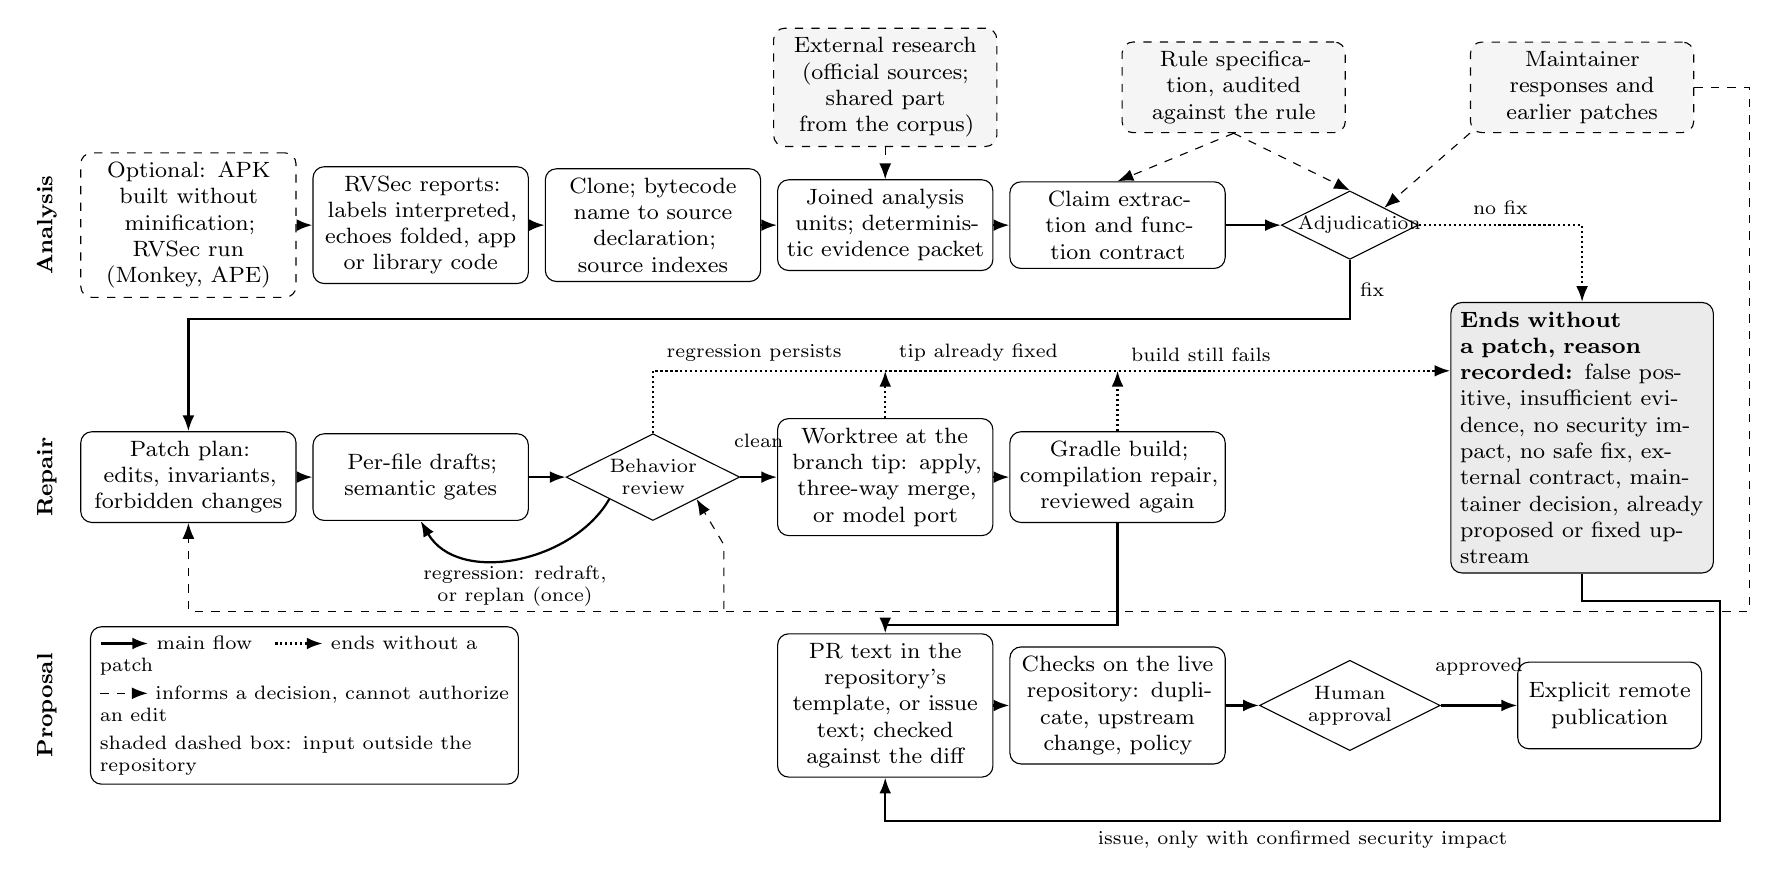
\begin{tikzpicture}[
  box/.style={draw,rounded corners,align=center,minimum height=11mm,
              text width=2.5cm,font=\footnotesize},
  opt/.style={box,dashed},
  inp/.style={draw,dashed,rounded corners,align=center,minimum height=8mm,
              text width=2.6cm,font=\footnotesize,fill=black!4},
  gate/.style={draw,diamond,aspect=2,align=center,font=\scriptsize,
               inner sep=0pt,text width=1.3cm},
  stop/.style={draw,rounded corners,align=left,font=\footnotesize,
               text width=3.1cm,fill=black!8},
  flow/.style={-{Latex[length=2mm]},thick},
  fail/.style={-{Latex[length=2mm]},thick,densely dotted},
  feed/.style={-{Latex[length=2mm]},dashed},
  lbl/.style={font=\scriptsize,align=center},
  lane/.style={font=\footnotesize\bfseries,rotate=90,anchor=south}
]
\def\cx#1{#1*2.95}
% ---------------- lane 1: analysis
\node[opt] (rvrun)  at (\cx{0},0) {Optional: APK built without minification; RVSec run (Monkey, APE)};
\node[box] (reports) at (\cx{1},0) {RVSec reports: labels interpreted, echoes folded, app or library code};
\node[box] (map)    at (\cx{2},0) {Clone; bytecode name to source declaration; source indexes};
\node[box] (units)  at (\cx{3},0) {Joined analysis units; deterministic evidence packet};
\node[box] (claims) at (\cx{4},0) {Claim extraction and function contract};
\node[gate] (adj)   at (\cx{5},0) {Adjudication};
\draw[flow] (rvrun)--(reports);
\draw[flow] (reports)--(map);
\draw[flow] (map)--(units);
\draw[flow] (units)--(claims);
\draw[flow] (claims)--(adj);
% inputs
\node[inp] (research) at (\cx{3},1.75) {External research (official sources; shared part from the corpus)};
\node[inp] (spec)     at (\cx{4.5},1.75) {Rule specification, audited against the rule};
\node[inp] (memory)   at (\cx{6},1.75) {Maintainer responses and earlier patches};
\draw[feed] (research)--(units);
\draw[feed] (spec.south)--(claims.north);
\draw[feed] (spec.south)--(adj.north);
\draw[feed] (memory.south west)--(adj.north east);
% ---------------- outcome without patch
\node[stop,minimum height=26mm] (stop) at (\cx{6},-2.7) {\textbf{Ends without a patch, reason recorded:} false positive, insufficient evidence, no security impact, no safe fix, external contract, maintainer decision, already proposed or fixed upstream};
\draw[fail] (adj.east) -| node[above,lbl,pos=0.25]{no fix} (stop.north);
% ---------------- lane 2: repair
\node[box] (plan)   at (\cx{0},-3.2) {Patch plan: edits, invariants, forbidden changes};
\node[box] (drafts) at (\cx{1},-3.2) {Per-file drafts; semantic gates};
\node[gate] (review) at (\cx{2},-3.2) {Behavior review};
\node[box] (tip)    at (\cx{3},-3.2) {Worktree at the branch tip: apply, three-way merge, or model port};
\node[box] (build)  at (\cx{4},-3.2) {Gradle build; compilation repair, reviewed again};
\draw[flow] (adj.south) -- ($(adj.south)+(0,-0.75)$) node[right,lbl,pos=0.5]{fix} -| (plan.north);
\draw[flow] (plan)--(drafts);
\draw[flow] (drafts)--(review);
\draw[flow] (review)--node[above=7pt,lbl]{clean}(tip);
\draw[flow] (tip)--(build);
\draw[flow] (review.south west) to[out=-120,in=-60] node[below=-1pt,lbl]{regression: redraft,\\or replan (once)} (drafts.south);
% failure exits (dotted) to the outcome box
\coordinate (bus) at ($(stop.west)+(0,0.85)$);
\draw[fail] (review.north) |- (bus);
\draw[fail] (tip.north) -- (tip.north |- bus);
\draw[fail] (build.north) -- (build.north |- bus);
\node[lbl,anchor=south west] at ($(review.north |- bus)+(0.05,0)$) {regression persists};
\node[lbl,anchor=south west] at ($(tip.north |- bus)+(0.05,0)$) {tip already fixed};
\node[lbl,anchor=south west] at ($(build.north |- bus)+(0.05,0)$) {build still fails};
% memory also informs planning and review
\draw[feed] (memory.east) -- ++(0.7,0) |- ($(plan.south)+(0,-1.12)$) -- (plan.south);
\draw[feed] ($(review.south)+(0.9,-1.12)$) -- ($(review.south)+(0.9,-0.3)$) -- (review.south east);
% ---------------- lane 3: proposal
\node[box] (text)    at (\cx{3},-6.1) {PR text in the repository's template, or issue text; checked against the diff};
\node[box] (checks)  at (\cx{4},-6.1) {Checks on the live repository: duplicate, upstream change, policy};
\node[gate] (approve) at (\cx{5},-6.1) {Human approval};
\node[box,text width=2.1cm] (publish) at (\cx{6}+0.35,-6.1) {Explicit remote publication};
\draw[flow] (build.south) -- ($(build.south)+(0,-1.3)$) -| (text.north);
\draw[flow] (text)--(checks);
\draw[flow] (checks)--(approve);
\draw[flow] (approve)--node[above=7pt,lbl]{approved}(publish);
\draw[flow] (stop.south) -- ++(0,-0.35) -- ++(1.75,0) |- ($(text.south)+(0,-0.55)$) node[below,lbl,pos=0.75]{issue, only with confirmed security impact} -- (text.south);
% legend
\node[draw,rounded corners,align=left,font=\scriptsize,anchor=west,text width=5.2cm] at (\cx{0}-1.25,-6.1)
 {\tikz\draw[flow](0,0)--(0.6,0); main flow\quad \tikz\draw[fail](0,0)--(0.6,0); ends without a patch\\[2pt]
  \tikz\draw[feed](0,0)--(0.6,0); informs a decision, cannot authorize an edit\\[2pt]
  shaded dashed box: input outside the repository};
% lane labels
\node[lane] at (\cx{0}-1.55,0) {Analysis};
\node[lane] at (\cx{0}-1.55,-3.2) {Repair};
\node[lane] at (\cx{0}-1.55,-6.1) {Proposal};
\end{tikzpicture}
}
\caption{Workflow exposed by the Python library and CLI. Solid arrows are the
main flow; dotted arrows end a unit without a patch, with its reason recorded,
and only a confirmed security impact turns such an end into an issue. Dashed
inputs inform decisions but cannot authorize an edit: only repository evidence
and explicit policy can.}
\label{fig:pipeline}
\end{figure*}

\subsection{From an RVSec Report to Source}

A data table in \system{} states what each RVSec label asserts: a value the
check does not admit, calls out of the rule's order, an origin the monitor did
not observe, an observed origin it does not admit, or an echo of a report about
the object's producer. An echo is folded into the findings of the method it
repeats unless its origin lies elsewhere. A finding is marked as application or
library code from the app's own packages (the namespaces of every module in the
repository); reports on obfuscated class names are set aside. When \system{}
starts the RVSec run, the APK is built without minification where the F-Droid
recipe allows, so runtime locations map back to source. The runtime observation
stays in the evidence, and its label bounds what the report establishes: an
unobserved origin states what the monitor saw, not what the object is---an IV
generated by the cipher provider is random although the monitor cannot trace
it.

The workflow clones the repository, records the documented base branch, reads
its guidance files, and maps the bytecode method to a source declaration.
Kotlin value-class mangling and compiler suffixes are removed; a lambda or
coroutine body that names no source function maps to the one function of its
outer class that uses the governed API or, failing that, to the one function it
calls in the same Gradle module that does; a method missing from the resolved
file is sought in the package's other files; and in Kotlin Multiplatform the
Android source set is preferred to desktop or iOS code the APK never contains.
An ambiguous match stays unresolved instead of guessed. Conservative
Tree-sitter~\cite{treesitter} indexes of Java and Kotlin supply the exact method, class context,
callers, overrides, references, value consumers, tests, dependencies, minimum
SDK, and Gradle configuration; relations that need a full JVM classpath stay
explicitly ambiguous. Target source is never truncated; a budget limits
auxiliary context and records every exclusion.

Findings in one piece of code form one unit with one patch: same class and
file, and either one method calls the other, one method violates two rules, or
one rule and message recur along one object's lifecycle. Findings of one
specification in different classes of a module also join when one method
stores a value the other reads back, such as an IV written at encryption and
read at decryption. Separate drafts for such findings rewrote the same code in
incompatible ways. A unit ends before any model call when each finding already
has a pull request of ours that is open or was merged after the analyzed
revision, or when the reported file is not on the target branch.

A fix may have to reach beyond the reported method. For each unit the index
lists the files a change could affect: callers in other files, overrides,
consumers of a shared symbol, related tests, configuration, and, when the
protected value is stored, every reader and writer of the same stored key and
every file the value flows through. A multi-file fix is applied without a
reader (\texttt{MULTI\_FILE\_FIX\_SUPPORTED}) only when this scope is complete,
adjudication reviewed every listed file, every file it marks for editing is in
the plan, and the patch edits at least two files. Short of that, the authority to apply
only goes down: when the index was truncated, a generic name stayed
unresolved, a listed file went unreviewed, or the plan edits beyond the
reported method, the decision becomes
\texttt{MULTI\_FILE\_FIX\_}\allowbreak\texttt{PROPOSED\_FOR\_REVIEW}, and the
unreviewed files are listed for the person who approves it; a decision that
is not review-only and lacks a required file generates no patch. Each file is
drafted separately against its siblings' declared interface, and a failed
check regenerates only the files it names. BitBanana's stored-verifier
migration shows the risk: an early candidate compiled while missing credential
readers (\researchq{2}).

\subsection{Specifications and External Research}

Each rule family has a JSON specification of governed types, events, detector
and runtime semantics, known false-positive shapes, and evidence requirements,
separating what a detector message asserts from what would establish runtime
harm (a literal \texttt{TLS} warning does not reveal the negotiated protocol).
Specifications are written by a model from the rule and official documentation
and audited deterministically against the cited rule, so a dropped event or an
added value is visible before it shapes an analysis.

Four specifications also carry curated remediation policies; with an
operator file that can set a policy per finding or finding family, they are the
explicit policy that can authorize an edit. Where a policy has variants,
deterministic evidence from the reviewed code, and from the hosts and files it
names, selects among them, and the resulting policy gives adjudication and
planning the scope, strategy, forbidden changes, and tests. A complete
multi-file plan awaiting policy is applied without further review only when the
policy authorizes it and the protected data is shown to stay in memory;
otherwise it is review-only.

Optional external research is a separate model call restricted to official and
primary sources; web or repository content is untrusted data that cannot
instruct the pipeline, choose files, or authorize publication. Its shared part,
about the API and rule, is kept in a research corpus and reused for up to 90
days only by a byte-identical request (same prompts, schema, model, effort,
output limit, and search tool); the case part is always researched. The case
study and published pull requests predate the corpus; the comparison's runs
record the state they started from (Section~\ref{subsec:frozen}).

\subsection{Evidence Packet and LLM Contracts}

Python builds an evidence packet per unit; each item has an identifier,
provenance, trust level, completeness state, and hash. Runtime observations and
exact source outrank semantic relations, official documentation, primary
research, secondary sources, and model inference. Absence is
\texttt{not\_found\_in\_examined\_scope}, \texttt{confirmed\_absent}, or
\texttt{unknown\_due\_to\_}\allowbreak\texttt{incomplete\_scope}, never used
interchangeably. Six model contracts follow:
(1)~\emph{evidence extraction} classifies claims as confirmed, inferred,
hypothesis, or unknown, citing evidence IDs, and states the code's function
contract---its purpose, its counterpart (a third-party service, a peer the user
operates, or the same app or device), and whether that counterpart depends on
the reported behavior, quoting repository code outside the reported method
verbatim; (2)~\emph{adjudication} decides cause, violation, runtime security
impact, compatibility, scope, generation and publication blockers, and the
disposition; (3)~\emph{planning} authorizes every file, symbol, edit kind,
invariant, and test, without code; (4)~\emph{generation} returns exact
per-file replacements; (5)~\emph{behavior review} reads the finished patch
against the whole file and the plan's invariants and forbidden changes, and
answers every adjudication concern; (6)~\emph{proposal text} describes the
final diff. When extraction names missing evidence or adjudication abstains for
lack of it, Python fetches it and both run once more, keeping the new answer
only if it validates. Narrower schema-checked stages handle research,
compilation repair, and the port to the branch tip.

Adjudication chooses among fifteen decisions in five groups: repairs applied
and built without further review (single- or multi-file fix, internal digest
migration, dependency fix or replacement); repairs a person must read before
application (multi-file fix, backend or multi-repository migration); decisions
awaiting explicit policy; confirmed violations needing no change here
(non-security digest use, no security impact, or an external digest contract
no client-side change can meet); and \texttt{NO\_SAFE\_FIX}. A review-only patch
is still built and reviewed; it becomes publishable only after a passing build,
a commit, and a current behavior review with no regression or blocker, and,
like every proposal, only with the author's approval.

A deterministic rule can also raise a \texttt{NO\_SAFE\_FIX} answer, or a
multi-file one awaiting policy, to the review-only
\texttt{MULTI\_FILE\_FIX\_}\allowbreak\texttt{PROPOSED\_FOR\_REVIEW}, never to a
decision applied without review, when the violation was not found false and
every generation blocker is either a question a reader of the patch settles (a
maintainer's authorization, device behavior, compatibility of stored data or
of a consumer) or evidence the packet lacked. A cause the source reading left
open then rests on the runtime observation or, for an echo, on its producer's
report, and a review assumption records this; the remaining generation
blockers become publication blockers, and the result must pass the same
validation. A confirmed repair rejected only for claiming generation while a
question of that kind stayed open is likewise kept for review instead of being
closed as \texttt{NO\_SAFE\_FIX}.

\subsection{Deterministic Safeguards and Residual Trust}

Deterministic checks guard each transition, because structured output does not
make a conclusion true. A confirmed claim citing an unknown evidence ID is
rejected; a supported adjudication needs a confirmed cause and detector
violation (in one raised to review-only, the cause may rest on the runtime
observation or a producer's report); a plan must cover every file the scope requires, and each generated
file must match a plan entry. Each replacement must occur exactly once in the
base source; unauthorized paths, unsupported edit categories, incomplete
coordinated edits, and cross-file symbol inconsistencies are rejected; build,
dependency, public-interface, and new-file edits need explicit categories.
Semantic gates reject known failure shapes: changing a stored, transmitted, or
constant-compared value without keeping the old form for existing data; leaving
a reader of a changed stored value unchanged; removing ciphertext the app
ships; replacing a protocol-mandated algorithm; or leaving the reported value
untouched. Each rejection returns to the generator with the reason; when no
in-app change can satisfy it (ciphertext under a shipped key), the finding goes
to the maintainers by the routing below. Checks over behavior a maintainer may
have chosen (removing or emptying a user setting or option, overriding or
refusing a value the caller supplies) do not refuse the patch: they become
notes shown to the author before approval, and the behavior review still
counts an emptied option as a regression. A rename must update every reference
in the same patch, or is regenerated with the failure explained; whether to
authorize it is a note in the pull request, not a block.

Trust remains: the index is not a complete JVM analysis, a resolved call may
depend on dispatch, reflection, or generated code, and documentation describes
an API contract, not the deployed provider. Unresolved assumptions stay
visible as \emph{review assumptions} for a maintainer or test, distinct from
\emph{generation blockers} (code would be unsupported) and \emph{publication
blockers} (buildable locally, not presented as ready).

\subsection{Behavior Review and Routing}

A regression needs a concrete scenario reachable through the application's own
code. Removing something deprecated or insecure offered to or accepted from a
peer is hardening unless evidence shows who depends on it: the function
contract, an option in the code, other code handling that peer, or the
maintainers. The review attributes each regression to the plan (no draft
following it can avoid the scenario) or to the draft. A draft's slip is
redrafted on the same plan with the scenario as feedback, regenerating tests
whose production file that feedback changes. After the plan's last draft, or
two consecutive plan-caused regressions, the unit is replanned with the
scenarios as constraints---at most once for any reason; if the new plan is not
taken, the first plan's remaining drafts still run. The review and
deterministic checks also reject a patch in which the governed call still
receives the same material (a renamed constant, an
alias or factory around the same object, a key rebuilt from its own bytes or
re-encrypted under the same key); if only such rejections remain, the finding
closes as a violation without security impact. A change that alters the value,
such as \texttt{SSL} to \texttt{TLS}, still becomes a proposal.

Findings without a patch are routed by established security impact. A
confirmed violation stopped before any draft (no safe fix, no edit found, an
external contract) becomes an issue only when its impact was confirmed;
otherwise it is recorded as lacking a safe correction or as blocked by an
external contract, with the blocker. Code already using the API as documented
closes as a violation without security impact only with a non-security impact.
A failed generation keeps its issue unless every blocker is a check on the
pipeline's own drafts (a rename left half done, an invented symbol, the
reported value left untouched) or, when the adjudication left the maintainer no
question, on their form (a draft with no edits). Such a finding ends as a fix
never produced, with no issue for it, since no maintainer can answer for a
draft the pipeline refused; so does, under the same condition, a fix the
adjudication supported that stopped before any draft only because the analysis
left unreviewed files the pipeline computed as in scope. Each finding ends in
exactly one outcome:
ready pull request (or one already open); patch without pull request (not
applied, not built, or held); not applicable; fix refused before any draft or
never produced; issue for the application or a bundled library; confirmed
violation without safe correction; violation without security impact; external
contract; maintainer decision; recognized false positive; insufficient
evidence; or not analyzed.

\subsection{Memory Across Runs}

Maintainer responses, refreshed from GitHub, reach adjudication, planning, and
behavior review for findings of the same specification, so a rejected premise
is not proposed again and a finding whose pull request was closed is not
republished. Earlier attempts are read only when they reached a patch, so one
run's sampling does not become the next run's evidence; facts confirmed by a
deterministic signal (an import a passing build accepted) are data and never
change code or prompts. For evaluation, a run can start with no attempt
history.

\subsection{Application on the Branch Tip and Build}

The analysis reads the APK's revision, but a pull request targets the base
branch's current tip. Each accepted solution is applied atomically in a
dedicated Git worktree at the tip, never in the base clone, with a distinct
path per attempt and a record of base commit, edits, and failure reason. The
literal edits are tried first, following renamed files, then Git's three-way
merge from the analyzed revision. Only if both fail does a narrow model stage
port the patch, given the reviewed patch, the upstream changes, and the tip's
files: it re-anchors the correction, states that the tip no longer contains the
violation, or declines. A port must pass the semantic gates and anchor checks;
new lines are reviewed for behavior again, and a rejected port returns once
more with the reason; a port the gates refuse while the violation remains
becomes an issue candidate. An already-fixed claim is accepted only when a
deterministic check confirms that the reported statement is in no file of the
tip, or that every corrected block is present and the replaced code is not;
otherwise it is a declined port. A finding is \emph{not applicable}, with no
pull request, when the tip holds the correction, the file left the branch, or
no port applies and the replaced code exists only at the analyzed
revision---nothing left to patch as reviewed, not a vanished violation. The
summary is rewritten after a port.

The build runs the selected Gradle task, normally a non-minified debug
assembly, on a JDK chosen from the wrapper and declared Java version, recording
commands, return code, APKs, logs, and diagnostics. SDK, JDK, Gradle, network,
or submodule failures are infrastructure failures; a failure the unmodified tip
shares is the project's but never a pass. Narrower passes (only the patched
module, only production code, or compiled on the analyzed revision because the
tip does not build) keep their own statuses and never count as a full build. A
patch in a source set the APK does not compile is not published. A narrow
compilation-repair stage may fix new diagnostics in changed files; it cannot
reopen the security decision, and edits outside the plan are reviewed again.
Where a static rule exists for the specification, it is re-run before and after
the patch as a measurement. These checks show the patch applies and builds, not
that it removes the runtime violation or preserves behavior; whether the
violation still appears is checked by the dynamic validation of published
pull requests (Section~\ref{subsec:dynval}).

\subsection{Proposal and Publication}

The text is written for the maintainer, not as a pipeline report. A model
drafts it from the final diff and the review's facts in a fixed shape: a title
that names the change, a few plain paragraphs on what the code did, what
changed, and whether it builds, and a fixed closing that names RVSec as the
analyzer and introduces the author. When the repository has a pull-request
template, the text fills it instead, keeping its headings and checklists and
ticking only verified boxes, such as a passing build, never a device test,
since RVSec ran the original APK. Deterministic checks then hold the draft to
that shape and to the diff: a generic title such as ``Fix \texttt{<init>}'',
evidence identifiers, compiled bytecode names, a summary over 250 words, terms
of the pipeline's own vocabulary, or a sentence describing an
edit absent from the final diff sends the text back for rewriting with the
problem stated, and publication is held only when the rewrite still fails.
The aim is a text in the project's terms, not one that hides its origin: AI
assistance is declared where a template asks. A \emph{ready pull request} is a committed
draft whose build passed: a candidate for human review, not a publication.

Nothing is published automatically: the operator approves each finding by its
identifier after a preview. \system{} then rechecks the live repository and by
default refuses a finding whose earlier pull request may be open or was closed
unmerged, a change another of its pull requests makes or overlaps, a diff the
default branch already contains or no longer matches, a test-only diff, a
review under an older contract, or a repository accepting no contributions;
each refusal names its override. An AI-contribution policy is reported to the
operator, who then writes the text; it does not block. An issue is refused when
its code left the default branch. \system{} never signs off another person's
commit; review comments are answered by revising the pull request, again after
approval. Creation targets GitHub; elsewhere the analysis and validated patch
are still produced. Prompt traces record requests, responses, versions, tokens,
and latency, never credentials.

\subsection{Inputs and Execution}

\system{} does not depend on one detector. A finding needs four fields (the
project, class, method, and violated specification) and may add the detector's
message, the repository, and the commit; findings are read from CSV, JSON,
SARIF, or Semgrep output, or produced by \texttt{cognalys scan}. For RVSec,
\texttt{cognalys fdroid-build} builds APKs without minification from their
F-Droid recipes, \texttt{cognalys github-build} does the same from the default
branch of an Android application on GitHub that has no recipe, and
\texttt{cognalys rvsec-run} runs RVSec with the chosen explorers and imports
its reports; instrumentation and the monitored
specifications stay in RVSec.

A run is started with \texttt{cognalys run} and a short configuration file.
Other commands, also available as a Python API (\texttt{cognalys.api}), list a
run's steps, summarize outcomes, report cost, show or apply patches, publish
approved proposals, and refresh maintainer responses.

Model calls go to OpenAI or Anthropic, or to a local model through Ollama, which
runs without web research. OpenAI calls use the Flex tier, priced at Batch API
rates~\cite{openai2026flex}; a call Flex cannot serve falls back to the standard tier, and the trace
records which tier answered. Two guards bound a run: it stops calling models at
a configured cost ceiling, and a model step with no call or log line for 30
minutes is stopped and resumed once from its response cache. Successful model
responses are cached across runs under a hash of the whole request, separately
from the research corpus.

\subsection{A Worked Example}

RVSec reported that \texttt{CryptoManager.getSecretKey} in Traffic Light
(version code 38) performed a call sequence that \texttt{KeyStoreSpec} does not
accept (the rule rejects a \texttt{getEntry} not followed by a
\texttt{getKey}~\cite{costa2026effectiveness}): it read the key with \texttt{KeyStore.getEntry} and took the secret key
out of the returned entry. \system{} mapped the method to its Kotlin source,
confirmed the violation and its cause, and judged its impact non-security: the
key is only read, and the app neither creates nor protects it differently.
Since a one-line change could bring the code to an accepted sequence, the unit
went on to repair. The draft replaced the lookup and kept the cache and the
fallback that creates a missing key; it passed the behavior review, applied at
the branch tip, and built.

{\scriptsize
\begin{verbatim}
- (keyStore.getEntry(key, null)
-     as? KeyStore.SecretKeyEntry)?.secretKey
+ (keyStore.getKey(key, null) as? SecretKey)
      ?: createKey(key)
\end{verbatim}}

The pull request (\#238), about 60 words in plain paragraphs naming RVSec as
the analyzer, was opened on October 20, 2026 and merged the next day with a
one-word reply. Rerun on the patched APK, RVSec no longer reported the
violation in the method in any of three runs (Section~\ref{subsec:rq7}). The
report disappears because the monitor now sees where the key came from, not
because the app became more secure: this is a confirmed violation without
security impact, which still becomes a pull request when its fix is safe.

\section{Study Settings}
\label{sec:settings}

The study has four parts with separate data and dates. (i)~A retrospective
case study of the 34 distinct findings in the consolidated snapshot of the
October 19, 2026 experiment, assembled on October 22 while the pipeline was
still changing (\researchq{1}, \researchq{2}, \researchq{4}, \researchq{5}).
(ii)~A survey of the 49 pull requests and 10 issues submitted for RVSec
findings, collected from GitHub on November 18, 2026 (\researchq{3};
Section~\ref{subsec:selection}). (iii)~A pre-registered, blind-judged
comparison of one recorded configuration of {\system} with coding agents in two
blocks, three arms given the finding and the repository and two instructed
to follow {\system}'s process, on 20 analysis units
(\researchq{6}; Sections~\ref{subsec:frozen} and~\ref{subsec:protocol}).
(iv)~A pre-registered dynamic validation that reruns RVSec on the original and
the patched APK of the published pull requests (\researchq{7};
Section~\ref{subsec:dynval}). Runs that preceded a registration, and every
deviation, are declared; later events do not rewrite an earlier build or
adjudication result. The four parts do not measure one system at one point in
time. The case study describes the pipeline as it stood in October 2026, with
an earlier model and several library revisions; the pull requests were
produced by the versions in use when each was opened, from August to November
2026; the comparison runs one frozen configuration with the current model; and
the dynamic validation reruns RVSec on the published pull requests, whichever
version produced them. Numbers are compared within a part, not across parts.

\subsection{Objectives and Research Questions}
\label{subsec:rqs}

The implementation objective is to complement runtime detection with
source-level classification, abstention, and reviewable repair through a
reusable library. The empirical objective is to describe what it decided,
built, and spent and how maintainers answered; to check with RVSec whether
published patches remove the violation; and to compare it with
general-purpose coding agents, with and without its process as instructions.

\begin{description}
  \item[\researchq{1}:] \emph{What analysis and repairability outcomes does
  {\system} produce for the selected API-misuse findings?}
  A proposal decision does not imply a generated or validated patch.

\item[\researchq{2}:] \emph{To what extent can the generated patches be
  applied to and compiled in the target projects?}
  We report application, build scope (APK or changed module), and failure
  attribution; this is buildability, not behavioral or security correctness.

  \item[\researchq{3}:] \emph{How do maintainers respond to submitted repair
  proposals, and what reasons do they give for their decisions?}

  \item[\researchq{4}:] \emph{Which detector reports does the analysis
  recognize as false positives or as violations without security impact,
  and are they concentrated in particular specifications?}

  \item[\researchq{5}:] \emph{How much model usage does the analysis
  require, and how is it distributed across outcomes?}

\item[\researchq{6}:] \emph{(a) Is a general-purpose coding agent enough when
  it receives the finding and the repository? (b) Does running the process as a
  pipeline add anything over an agent instructed to follow the same process?
  (c) How much do the deliveries of {\system} vary between runs?}
  One agent configuration uses {\system}'s model, so a difference between the
  two cannot be attributed to the model.

  \item[\researchq{7}:] \emph{When RVSec runs again on the patched APK of a
  published pull request, does the reported violation still appear in the
  patched method?}
  A build or a merge does not show that the observed misuse is gone.
\end{description}

The finding identity is APK identifier, class, method, and specification; the
pull-request identity is repository and pull-request number. Repeated attempts are not independent
cases; different specifications in one method remain distinct findings, even
when one patch addresses both. Pull-request status and build status are separate
dimensions. The case study and the survey are exploratory: no hypothesis was
fixed beforehand, and the pipeline changed meanwhile (each change is recorded
beside the measurement that motivated it). The comparison and the dynamic
validation follow procedures and analysis rules written down and dated
before their runs; the comparison's registrations also record the hashes of
its prompts, scripts, and answer keys. Each registration states which runs
preceded it, and every rule changed after results were seen is declared as a
deviation. No statistical test is applied: results are descriptive counts and
case explanations (Table~\ref{tab:rq-data}).

\begin{table}[tb]
\centering
\caption{Data behind each research question.}
\label{tab:rq-data}
\footnotesize
\begin{tabular}{p{0.9cm}p{3.7cm}p{2.6cm}}
\toprule
RQ & Data & Units and date \\
\midrule
RQ1, RQ4 & Case study: consolidated snapshot of the October 19 experiment & 34 findings, Oct.~22 \\
RQ2 & Case study: generated fixes, application at the tip, and builds & 11 fixes, 7 built \\
RQ3 & GitHub survey of pull requests and issues for RVSec findings, three origins (Table~\ref{tab:origin}) & 49 PRs, 10 issues, Nov.~18 \\
RQ5 & Prompt traces of the case study's runs & 34 findings, 11 runs \\
RQ6 & Comparison with coding agents (registered in advance) & 20 units (24 findings), 4 runs per unit \\
RQ7 & RVSec on original and patched APKs (registered in advance) & 45 of 49 PRs, Nov.~14--19 \\
\bottomrule
\end{tabular}
\end{table}

\subsection{Case Selection}
\label{subsec:selection}

\subsubsection{Dated case study and pull-request survey}

The case study holds 34 distinct findings from 23 APKs, each with the
repository and source commit of its APK. The findings come from the RVSec
group's campaign over 163 F-Droid applications~\cite{costa2026effectiveness}.
In the campaign's data, of the 109 uses selected for source-level follow-up, 72 lay in library
code absent from the repository at the analyzed commit, three in a vendored
copy of a library, and 34 in the application's own code (31 misuses the
campaign established and three seen in a single run, which it left undecided). The case study joins a base run and later
targeted reruns, keeping each finding's latest outcome, so it holds 34
findings rather than 34 independent executions, and it describes what the
October 2026 version decided, built, and spent, not what the current version
would decide; \researchq{6} measures the frozen configuration of
Section~\ref{subsec:frozen}. These runs kept the response cache, so a model
request identical to one answered before was served from it rather than
sampled again (for web research, only within a week).

Pull-request states and responses were collected from the GitHub API on
November 18, 2026. Inclusion requires an open pull request, an incorporated change, or closure
by a maintainer; superseded attempts closed by the author or a bot are
excluded. BombusMod \#316 is manual incorporation, not a GitHub merge.

A pull request counts as RVSec when its finding comes from an RVSec report,
traced through the run that produced the pull request. The pull requests and
issues have three origins (Table~\ref{tab:origin}). The data of the RVSec group's
campaign~\cite{costa2026effectiveness} supply the 34 findings of the case
study; eight pull requests and three issues come from runs on its data after
September 16, 2026. Our own runs from August 8 to September 16, 2026, on RVSec
reports that predate the campaign, produced 15 pull requests and five issues;
eight of these pull requests address case-study findings, which the campaign
reported again, and are linked to them by finding identity. Our RVSec queues
produced the other 26 pull requests (opened October 16 to November 7) and two
issues: each application ran once under RVSec with Monkey and APE for 600
seconds, with the cryptographic and TLS specifications, and only findings in
the application's own code were analyzed. Queue candidates were F-Droid
applications and, later, Android applications on GitHub without an F-Droid
recipe, preferring those whose cryptographic code runs without an account;
later still, their repositories also had to be active and to have merged a
pull request from an outside contributor in the previous twelve months.

\begin{table}[tb]
\centering
\caption{Origin of the pull requests, issues, comparison units, and
dynamic-validation cases. Pull requests and issues are assigned by the run
that produced them, comparison units by the source of their finding. States
on November 18, 2026: incorporated/closed/open. RQ7: cases run/labeled
corrected.}
\label{tab:origin}
\footnotesize
\setlength{\tabcolsep}{3pt}
\begin{tabular}{p{3.0cm}rcrrc}
\toprule
Origin & PRs & Inc./Cl./Open & Issues & RQ6 & RQ7 \\
\midrule
Our runs on earlier RVSec reports (Aug.~8--Sep.~16) & 15 & 6/4/5 & 5 & 0 & 12/6 \\
RVSec group's campaign (after Sep.~16) & 8 & 4/1/3 & 3 & 10 & 7/5 \\
Our RVSec queues (Oct.~16--Nov.~7) & 26 & 11/5/10 & 2 & 10 & 26/22 \\
\midrule
Total & 49 & 21/10/18 & 10 & 20 & 45/33 \\
\bottomrule
\end{tabular}
\end{table}

Table~\ref{tab:sample} gives the inventory.

\begin{table}[tb]
\centering
\caption{Case inventory and overlap (PR and finding counts use different units).}
\label{tab:sample}
\footnotesize
\begin{tabular}{p{6.1cm}r}
\toprule
Inventory component & $n$ \\
\midrule
Consolidated findings & 34 \\
Eligible published PR records & 49 \\
PR records with a complete finding identity & 48 \\
Overlapping findings retained once & 15 \\
Additional fully linked PR findings & 32 \\
\quad from our RVSec queues & 26 \\
\quad from our earlier runs & 6 \\
Fully linked finding union & 66 \\
Distinct APK identifiers in that union & 53 \\
PR records with incomplete source links & 1 \\
\bottomrule
\end{tabular}
\end{table}

Matching uses the full finding tuple and the published URL, feedback identity,
or source metadata, never repository membership alone; unresolved links stay
visible rather than receiving invented identities. The 48 records with a
complete identity correspond to 47 findings, 15 overlapping the case study,
so the union holds 66 findings from 53 APK labels. HTTP Shortcuts \#576,
lacking a complete APK/class/method/specification link, stays in the PR
inventory but out of those denominators. Selection is purposive (cases
actually analyzed or submitted, including negative feedback), not a
representative sample. Forty-six of the 49 pull requests concern
cryptographic specifications (HTTP Shortcuts \#576's, \texttt{SSLContextSpec},
was recovered from a recorded source for \researchq{7}); three (BombusMod,
wwwjdic, and ntfy), from our earlier runs, concern resource-handling and
synchronization specifications that our queues do not enable. Fourteen pull requests for manually
identified candidates, web research, and Semgrep rules, submitted during
development, are reported apart as an extra and left out of every count: on
November 18, 2026, five were incorporated (aiHub \#279, HomeApp \#114,
Auto-Shine \#12, SlimBook \#3, and aaf-easydiary \#253), two were open, and
maintainers closed seven.

\subsubsection{APK and revision provenance}

RVSec observes an APK, but \system{} patches a commit, so each finding
records the repository and commit of its APK. Of the 26 of the 53 APKs whose
binary is still available, the manifest matched for 22; the other four are
debug builds whose package carries a variant suffix (\texttt{.dev},
\texttt{.staging}, \texttt{.debug}), two also with a different version code.
For the other 27 the correspondence is assumed
(Section~\ref{subsec:threats}). The queues' applications from GitHub without an
F-Droid recipe were built from the head of their default branch; three of the
49 pull requests come from them (TriliumDroid \#177, meshcore-mobile-app \#10,
and CometOTP \#114). All repositories are on GitHub, whose API is used both to
publish and to collect responses. When the base branch has moved, the
patch is carried forward before a pull request is opened
(Section~\ref{sec:pipeline}).

\subsection{Procedures for Data Collection}
\label{subsec:collection}

\begin{table}[tb]
\centering
\caption{Principal collected artifacts.}
\label{tab:artifacts}
\footnotesize
\begin{tabular}{p{2.3cm}p{5.0cm}}
\toprule
Artifact & Information used in the study \\
\midrule
Extracted method & Finding metadata, exact source, imports, call sites,
specification context, repository guidance \\
Evidence packet & Stable evidence IDs, provenance, trust, relations,
ambiguities, exclusions, completeness, hashes \\
Adjudication & Cause and impact states, decision, blockers, supporting claims,
required tests \\
Patch plan/solution & Authorized files and edits, invariants, review status,
exact replacements \\
Execution report & Worktree/base commit, application status, changed files,
revision and errors \\
Build report & Task, status, return code, duration, diagnostics, logs and
failure attribution \\
Prompt trace & Stage, request/response, versions, tokens, latency, cache and
request identifiers \\
Judged card & Delivery kind, title, text, diff, build flag; judge scores and notes \\
RVSec rerun & Original and patched APK, violations and coverage at the patched method \\
\bottomrule
\end{tabular}
\end{table}

Each finding keeps the artifacts of Table~\ref{tab:artifacts}. For
\researchq{3}, we recorded for the 49 eligible pull requests and the 10 issues,
opened between August 8 and November 7, 2026 (the issues by November 5), their
state, merge, who closed them,
and whether anyone other than the author or a bot commented, reviewed, or
closed them (a maintainer response); issues are inquiries whether a pull
request would be welcome or reports of findings with no safe fix. The 23
issues opened on August 4, a test with a local model, are excluded
(Section~\ref{subsec:ethics}). For
\researchq{5}, each traced call records its model and input, cached-input, and
output tokens and is attributed to its finding; calls sent to a provider are
priced at list prices and summed per finding over the snapshot's runs of
October 19 and 20, 2026, leaving out calls
made for no finding and requests answered from the response cache, which cost
nothing. For \researchq{6}, each agent run keeps its delivery, diff, build
log, event log, and tokens, plus the port phase for a pull request; the
card-to-arm key is kept apart from the judges. For \researchq{7}, each case
keeps both APKs, the patched build record, and every RVSec report.

\subsection{Procedures for Data Analysis}
\label{subsec:analysis}

We keep each finding's latest outcome without pooling attempts, and pull-request status
and feedback separate from that snapshot; the machine-readable inventory keeps
source paths, matching basis, PR URLs, binary availability, manifest package,
and version. A build-valid proposal is not necessarily correct, secure,
accepted, or free of the detector's report (checked for published pull
requests in \researchq{7}, only on paths the explorers reach), and a closed
pull request is not necessarily a wrong patch (intentional behavior, policy, an
already-applied change, or manual incorporation). We therefore avoid a pooled
success rate. The outcomes of \researchq{1} and \researchq{4} are the
pipeline's recorded decisions; where the text calls a decision correct or not,
that is the author's reading of the run's evidence. The closure reasons of
Table~\ref{tab:closures} were coded by the author from each maintainer's own
words, one reason per pull request, without a second coder.

\subsection{Fixed Configuration and Units of the Comparison}
\label{subsec:frozen}

The comparison runs {\system} at one fixed configuration: a single library
version (four of its 80 runs, which had failed on implementation
defects, were rerun after those defects were fixed), \texttt{gpt-6.1-terra} for every stage at high reasoning
effort with a 32,768-token output limit, on the Flex tier, with every patch
built and a ceiling of US\$2 per run. A run counts only when its experiment
manifest (model, prompts, schemas, policies, specifications, learning store,
research corpus, commit) matches. Three leak controls apply: the unit's own
repository is held out (neither its maintainers' responses nor what earlier
runs learned there reach any prompt, while other repositories' responses to
the same rule remain, and the second-block agents receive the same ones); the
learning store holds verified imports but no earlier attempt; and no response
from an earlier run is reused except the shared, rule-level web research from
the recorded corpus, the unit's own case being always researched again; within
a run, a request that a unit's analysis repeats verbatim, as in a replan,
reuses its first answer.

The model was chosen by a descriptive check: eight units (ten findings from
six applications) were rerun with \texttt{gpt-5.6-terra}, used until
November 2, 2026, and \texttt{gpt-6.1-terra}
under the same settings. Both made 83 calls, costing US\$6.31 and US\$2.43 at
list prices (US\$2.71 for \texttt{gpt-6.1-terra} with its cache-write price
and search fee); they agreed in four of the eight units. The sample is too small to compare decision quality;
the lower cost supported the change.

The 20 analysis units were drawn on November 13, 2026 with a recorded seed.
Ten come from published pull requests whose original run ended with a
committed, building draft, stratified by their state on that date: three incorporated, five
open, two closed by the maintainer. Ten come from the 45 distinct findings of the case
study (34) and of an earlier exploratory comparison with agents (12, one of
them shared), which the pipeline analyzes again, excluding methods that also
appear in the pull-request population of the first ten: nine without a
pull request and one whose pull request the maintainer closed. By origin
(Table~\ref{tab:origin}), ten units come from the RVSec group's campaign (two
of them among the pull-request units) and ten from our queues (eight). A unit is one finding, or
several findings the pipeline joins into a single patch
(Section~\ref{sec:pipeline}): four units join two findings each, two within one
method and two across two methods of one class.

\subsection{Comparison with Coding Agents}
\label{subsec:protocol}

\emph{Arms.} Five agent arms in two blocks are compared with {\system} (arm
C), in three configurations: the Codex CLI with \texttt{gpt-6.1-terra}
({\system}'s model), Claude Code with Claude Sonnet 5.5, and the Codex CLI
with \texttt{gpt-6.1-sol}. In the first block (T, S, O) each agent receives
the finding and the repository and delivers once, judged at the analyzed
commit without a port; in the second (TP, SP2) the first two configurations
also receive {\system}'s process as instructions and port their pull requests
to the branch tip. All run at high effort, four times per unit. T, TP, and C
share the model, so their differences reflect the instructions and where the
process runs (one session, or separate stages with deterministic checks
between them). A partial run of {\system} with Claude Sonnet 5.5 (17 of 40
planned runs) is not compared; its cards enter only the judges' agreement and
the first block's blinding probe.
A third second-block arm, with \texttt{gpt-6.1-sol}, was stopped after 25 of
its 80 runs, before any was judged, when the subscription quota ran out, and is
not compared (a declared deviation).

\emph{Phase 1.} Each run starts from a fresh checkout of the analyzed commit,
without remote, credentials, or memory, with a 60-minute limit, web search,
and {\system}'s build command. The prompt gives the RVSec report lines, asks
for exactly one delivery (pull request, issue, or nothing to send), and states
{\system}'s text rules. The second block's prompt adds each report's published
rule, other repositories' maintainer responses to it, and the inputs {\system}
reads, and describes each stage in order (evidence, research, decision,
planning, drafting, checks, behavior review, redrafting and replanning, build,
text). The Claude Sonnet arm's first version, SP, asked like TP for
stage-by-stage notes; the model's safeguards in Claude Code stopped most of its
runs, so SP2 uses the prompt without that request. A prompt
cannot reproduce separate contexts per stage, code-enforced validators and
retries, or the research corpus.

\emph{Phase 2.} As {\system} does (Section~\ref{sec:pipeline}), second-block
pull requests go to the unit's single tip, taken from the {\system} runs: a
three-way merge first, built without the agent when clean; on a conflict, the
same agent, model, and effort report the patch as ported, already fixed, or
abandoned. ``Already fixed'' stands only when a deterministic check finds the
added lines present and the removed lines absent at the tip; otherwise it is
abandoned. Both phases' tokens count toward cost.

\emph{Cards and judges.} Each delivery becomes a card (kind, title, text,
diff against the analyzed commit, build flag) stripped of signatures,
identifiers, tool names, and pipeline vocabulary, enforced by a lint. Two
judges, Claude Opus 5.5 (principal) and \texttt{gpt-6.1-sol}, at high effort,
without web access, with a read-only checkout, score every card of a unit in
random order, since the order in which candidates are shown can change a
verdict~\cite{wang2024fair}. The scores are patch 0 (reject) to 3 (mergeable as is), text
accuracy 0 to 2, and the reason for an issue or abstention 0 to 2. The final
score is the agreed one, or Opus's when they differ. A model tends to favor
its own generations~\cite{panickssery2024selfpref}, and each judge is close to
some arms: GPT-6.1 Sol is O's model and comes from the provider of T's, TP's,
and {\system}'s, while Claude Opus 5.5 comes from S's and SP2's, so the
agreement between the judges is reported beside the final score. Scoring follows a
written reference per unit (what an acceptable patch must change and must not
break), drafted by the judges and written without any maintainer response.

\emph{Acceptability.} A run is acceptable when it delivers an issue or an
abstention, or a pull request with patch at least 2 and text at least 1,
built at the tip after the port (first block: at the analyzed commit); a
build failure the unmodified code shares is not charged to the patch. A pull
request whose port found the fix already at the tip, or was abandoned, is
never sent and is judged on its patch alone (at least 2); this rule was set
after results were seen and is declared as a deviation.
A failed run counts 0. An arm's measure is the share of acceptable runs per
unit, averaged over units, under two readings: the full reading judges the
whole card as above, and the patch-only reading hides title and description
(acceptable: patch at least 2 and built; issues and abstentions unjudged and
acceptable). For {\system}, a pull request is any generated fix, the unit counted in
\researchq{1}: a committed draft, even one the pipeline would hold back, which
must build at the tip unless the tip already held the fix or no longer had the
code (it is then judged on its patch alone). Because issues and abstentions always
count, the measure rewards abstention (an arm that never proposes scores 1),
so we also report per arm the pull requests proposed, judged acceptable, and
judged unacceptable (proposed minus acceptable), and the units with at least
one acceptable pull request. ``Acceptable'' is the judges' verdict, not a
maintainer's.

\emph{Blinding.} A separate principal-judge session, given one card at a
time, tries to name its arm on full and patch-only cards, reporting its
overall and per-guess accuracy. It ran on the first block's and {\system}'s
cards and, before any second-block score was read, on 10 cards per arm of TP,
SP2, and {\system} in each view (a declared addition).

\emph{Cost and analysis.} Cost is a reference, not a criterion: agents are
priced at list prices with the web search fee (the agents ran on subscriptions,
so this is what the same tokens would cost through the API), and {\system} at what the
Flex tier billed and at list price. With 20 units and four replicas no
statistical test is applied; we report the final scores, the judges' agreement
(Cohen's kappa), and observed differences. RVSec does not enter the scores, since only
{\system}'s published patches were rerun (\researchq{7}).

\subsection{Dynamic Validation of Published Pull Requests}
\label{subsec:dynval}

The procedure of \researchq{7} was registered on November 15, 2026, before any
new case was built or run; it extends a pilot on the six snapshot previews that built an APK, an extension
decided after the pilot's results were known. Of the 49 pull requests of
Table~\ref{tab:pr-state}, sixteen are excluded with a recorded reason:
specification outside the cryptographic and TLS set RVSec checks (three), no
recorded identity or pipeline metadata, no matching detector line at the
reported method, no build producing the analyzed APK, or a pull request
addressing a different finding. The remaining 33 are 28 new cases and the five
pilot cases whose validated patch is the published pull request (four
corrected and BitBanana, inconclusive), which the pilot had run three times
with the same RVSec settings (the pilot used a fixed JDK; new cases choose it
as the pipeline does). The pilot's PassNotes case checked a finding and patch other
than those of keepassvault \#347, which was added later as its own case.

The original and patched APK are built from the same commit and Gradle task,
without minification; the patch is the pull request's public diff at its
merge base, or the pipeline's diff when identical. RVSec runs on each APK in a
clean emulator for 600 seconds, with Monkey and APE and its cryptographic and
TLS specifications. Every case gets one repetition, and an inconclusive or
non-reproducing case a second, time permitting. A failing build is retried
once, then reported as not built, as is a patch that does not apply; the
application's code is never edited. Labels follow a rule fixed before the
runs: \emph{base does not reproduce} (left out of the count) when the original
APK shows no violation of the specification at the method in any repetition;
otherwise \emph{not corrected} when the patched method reports one in any
repetition, \emph{corrected} when it executes without one, and
\emph{inconclusive} when it never executes. Results read ``the reported
violation no longer appears in the patched method'', not ``RVSec no longer
reports the application''. Cases not finished by November 18, 2026
(November 19 for the six recovered pull requests and the extra repetitions
described below) are reported as not
executed.

\emph{Review of labels.} After the runs, every label other than \emph{corrected}
was reviewed against the runs, the pull request's diff, and the original
source, and corrected where the rule's label misdescribed the case; the rule's
label is kept beside it. When the patched method never executes, the case is
\emph{corrected} if the patch removed the governed call from its file or turned
off, by default, the condition guarding every call of the method, and \emph{not
corrected} if the reported violation appears at another method of the same
file. A reported message that disappeared, leaving at the method only messages
of the specification the original APK already showed, is \emph{corrected}; a
pull request that changes only tests is labeled as such. A case is \emph{not
verifiable} when the reported violation appears in neither APK and its message
is emitted by no run of the validation: the report came from an RVSec rule set
older than the campaign's.

\emph{Additions after the registration.} The following steps were not part of
the registered procedure. The FreeOTP finding, one of the case study's, came from
the RVSec group's campaign~\cite{costa2026effectiveness}; in the campaign's
original report, only DroidBot, Humanoid~\cite{li2019humanoid}, and
ARES~\cite{romdhana2022ares} reached the method, so its two pull requests are
also run with DroidBot, one of the original report's explorers, for 300
seconds and three repetitions, beside the Monkey and APE results (Humanoid and
ARES could not run here). Inconclusive cases and cases whose original APK did
not reproduce the violation got one more repetition, labeled with all
repetitions together: a third for Read You \#1334, Your Local Weather \#209,
InterTune \#52, and News \#1716, and a fourth for BitBanana, inconclusive in
the pilot; in Your Local Weather the original APK showed the violation only in
the third. After the results of the 33 were known, 13 excluded pull requests
were added: seven whose recorded report used an earlier message format of
RVSec, which no current detector line matched, labeled by the specification
alone (any violation of it at the method counting), and six whose analyzed APK
or finding identity was recovered from the pipeline's records; twelve of them
were built and run with the current RVSec under the same settings. Of the 33 cases
labeled corrected in the end (Table~\ref{tab:dynval}), 27 were classified, 21
of them with a second, adversarial reading, as changing the
governed value or material, changing the call sequence or API to the required
form, removing the governed call, or only relocating it out of the monitor's
view; this classification is descriptive, and the six labeled corrected after
it were not classified (Section~\ref{subsec:rq7}). In all, 46 of the 49 pull requests
entered the validation: 45 were run, MetadataRemover \#264 does not build at
its base commit, and the three outside RVSec's set stay excluded.

\section{Results}
\label{sec:results}

\researchq{1}, \researchq{2}, and \researchq{4} use the October 2026
snapshot, and \researchq{5} the model usage of its findings: the 34 findings
of the experiment of October 19, 2026, with the outcome of each one's latest
run of the consolidated experiment (October 19 and 20); \researchq{4}'s
breakdown of pull requests by specification uses the November 18 survey of
\researchq{3}. Those runs used several
library revisions with \texttt{gpt-5.6-terra} on the standard tier, before the
frozen configuration (Section~\ref{subsec:frozen}) and several routing rules
(Section~\ref{sec:pipeline}): a dated case study of an earlier version, not a
measurement of the current one. \researchq{3} reports pull requests and issues
on November 18, 2026; \researchq{6} the comparison of
Section~\ref{subsec:protocol}; \researchq{7} the RVSec reruns of the published
pull requests, from November 14 to 19, 2026.

\subsection{\researchq{1}: Finding Analysis and Repairability}
\label{subsec:rq1}

The adjudication of the 34 findings recorded 17 decisions to propose a
reviewable fix (\texttt{MULTI\_FILE\_FIX\_PROPOSED\_FOR\_REVIEW}), 13 that no
safe fix existed (\texttt{NO\_SAFE\_FIX}), and four that an external digest
contract prevented a client-only fix. Table~\ref{tab:adjudication} shows
where each finding ended, as local records: an issue there is a proposal kept
for review; publication is a separate step, outside the snapshot's runs.

\begin{table}[tb]
\centering
\caption{Outcome of the 34 findings in the October 2026 snapshot (local
records).}
\label{tab:adjudication}
\footnotesize
\begin{tabular}{p{6.1cm}r}
\toprule
Recorded outcome & $n$ \\
\midrule
Generated fix & 11 \\
\quad committed at the branch tip and built\textsuperscript{a} & 7 \\
\quad applied; build failed, as on the unmodified base & 1 \\
\quad not applicable to the current base branch & 3 \\
Local issue proposal for the maintainers & 16 \\
Recognized false positive & 3 \\
Insufficient evidence & 3 \\
Confirmed violation without a safe fix & 1 \\
\midrule
Total & 34 \\
\bottomrule
\end{tabular}
\\[2pt]\raggedright\scriptsize\textsuperscript{a}Six to an APK; for Feeder only
the application module was compiled.
\end{table}

The three not-applicable fixes met a base branch that had already changed, in
two cases through this work's own merged pull requests, so none produced a pull
request in the snapshot. Nextcloud Cookbook's base held \#204 (merged on August
9, 2026). Giggity's maintainer had made an equivalent change independently and
closed \#543. In DSub2000 the reported method had been changed by \#160 (merged
on August 31, 2026), which addressed another message of the same rule, but the
base still initialized TLS with an accept-all trust manager; a check rejected
the adaptation because it removed what the user's insecure-connection option
turned on, and the port step abstained. A later run opened DSub2000 \#178 for
that trust manager on October 22; it was withdrawn the same day, after the
maintainer replied that skipping certificate checks is the purpose of that
option, and it is not among the 49 pull requests.

Six proposal decisions ended as issue proposals because generation was
blocked: the drafts needed production credentials the repository lacks (MTG
Familiar), changed a protocol-mandated algorithm (two in mOTP), changed
persisted database names (RedReader), overrode a caller-chosen RSA key size
(Droid SCEP), or called nonexistent verifier methods (BitBanana, whose
migration reached a pull request through its sibling finding): a positive
planning decision is weaker than a validated repair. The other ten came from
no-safe-fix or external-contract decisions; the current library opens an
issue for these only with a confirmed security impact
(Section~\ref{sec:pipeline}), which by the snapshot's records nine would lack.

Fifteen of the 34 findings also have a published pull request (16 pull
requests; Table~\ref{tab:sample}); on November 18, 2026, the pull requests of
five findings were incorporated, five closed, and five open, DSub2000 counting
as incorporated through \#160. Nine of these pull requests are not later
events: they were opened from earlier analyses of the same findings, before the
snapshot (August 8 to October 12, 2026), and six had already been merged or
closed when it ran. Later runs changed some outcomes. The FreeOTP
\texttt{CipherSpec} finding, without a safe fix in the snapshot, was analyzed
again in seven later runs, and FreeOTP merged a test (\#521) and then the
production fix (\#524). The test came from the first of these runs: its
adjudication left the cause open, and a deterministic rule, used by none of the
snapshot's runs, let the cause rest on RVSec's runtime observation and raised
the answer to the review-only
\texttt{MULTI\_FILE\_FIX\_}\allowbreak\texttt{PROPOSED\_FOR\_REVIEW}.
The production fix came from a later run whose adjudication confirmed the cause. The Droid SCEP issue proposal became pull request \#2. Six issues concern
these findings. Critical Maps (\#379, later closed by us, and \#380, still
open) and OpenBible (\#190) were opened in August, before the snapshot. MTG
Familiar \#669 and DSub2000 \#177, the latter on DSub2000's trust manager, came
on October 20 from a separate issue run outside the consolidated experiment,
and RedReader \#1394 followed on October 21.
For WiFiAnalyzer the snapshot declined a fix and recorded no security impact,
the maintainer's reason for closing \#618, yet still proposed an issue, which
the current routing would not; for RedReader's \texttt{sha1} it proposed a fix
whose premise the maintainer had rejected when closing \#1373.

\textbf{Answer to \researchq{1}.} In the October snapshot, 17 of the 34
findings had a decision to propose a fix and 11 reached a generated fix: seven
were committed at the branch tip and built, one applied but failed to build as
the unmodified commit also did, and three were not applicable because the base
had changed, two of them through this work's earlier pull requests. Sixteen
ended as local issue proposals (Table~\ref{tab:adjudication}). These are classifications of an earlier library version;
later runs and maintainer responses changed several of them.

\subsection{\researchq{2}: Application and Build}
\label{subsec:rq2}

The 17 proposal decisions yielded 11 generated fixes
(Table~\ref{tab:adjudication}): eight applied at the branch tip as local
pull-request previews, and three were not applicable to it. Seven previews were
committed and built, six to an APK (for Feeder only the application module's
sources were compiled). The eighth, MetadataRemover, fails in Hilt's
annotation processing with the same error on the unmodified commit.

An audit of the previews found concerns no build reveals: BetterUntis renames
persisted cache files without stating that compatibility decision, PassNotes
keeps an accept-all hostname verifier in its debug branch, and Feeder's
\texttt{trustAllCerts} validates certificates after the patch while keeping
its name. In BitBanana an early candidate compiled while omitting credential
readers affected by the new stored verifier; the October 20 delivery (a
helper and six credential screens) keeps legacy verification, replaces a
stored verifier only after a successful unlock, and built an APK. No
application flow was tested; \researchq{7} checks only whether the reported
violation still appears in the patched method at runtime.

\textbf{Answer to \researchq{2}.} Of the 11 generated fixes, eight applied at
the branch tip and seven of these built, six to an APK; the eighth fails on the
unmodified commit too, and three met a base that had already changed. The build
did not reveal the concerns the audit found in three previews.

\subsection{\researchq{3}: Maintainer Responses and Reported Reasons}
\label{subsec:rq3}

Table~\ref{tab:pr-state} gives the state of the 49 pull requests on November
18, 2026; 67\% received a response from someone other than the author. The
incorporated ones include BombusMod \#316, applied by hand, and FreeOTP \#521,
which only adds a test (the production change, \#524, was also merged). By the
origin of the run behind each pull request (Section~\ref{subsec:selection}), 8
come from the RVSec group's campaign (4 incorporated, 1 closed, 3 open), 15 from
our analyses of RVSec reports that predate it (6, 4, 5), and 26 from our own
RVSec queues (11, 5, 10); the split is descriptive, as the queues favored
repositories that accept outside pull requests.

\begin{table}[tb]
\centering
\caption{State of the 49 RVSec pull requests on November 18, 2026.}
\label{tab:pr-state}
\begin{tabular}{lr}
\toprule
State & PRs \\
\midrule
Incorporated (20 merged, 1 manually) & 21 \\
Closed after review                  & 10 \\
Open (16 without a reply)            & 18 \\
\midrule
Total                                & 49 \\
Received a maintainer response       & 33 \\
\bottomrule
\end{tabular}
\end{table}

Of the ten issues opened for RVSec findings (three for findings of the
group's campaign, five from our earlier analyses, two from our queues), two,
opened in September beside
the BombusMod and wwwjdic pull requests, asked whether maintainers would
welcome a pull request; neither received a reply, and we closed both. The other
eight described a finding with no safe fix and asked how to handle it; four
received a response and two remain open. Three of these answers supplied what
the rule could not know (a fallback kept for usability, users' self-signed
servers, a checksum algorithm set by a remote source), and the DNSToggle
maintainer fixed the finding in a release.

\begin{table}[tb]
\centering
\caption{Reasons given for the 10 pull requests closed without
incorporation.}
\label{tab:closures}
\footnotesize
\begin{tabular}{p{5.8cm}r}
\toprule
Stated reason & PRs \\
\midrule
Digest used outside a security role (checksum, cache or file name,
identifier) & 6 \\
Detector premise does not hold (provider already generates a random IV) & 1 \\
Change only satisfies the rule; existing code is equivalent & 1 \\
Equivalent change already made upstream & 1 \\
Project not accepting pull requests & 1 \\
\midrule
Total & 10 \\
\bottomrule
\end{tabular}
\end{table}

Maintainer responses add application knowledge a generic rule lacks
(Table~\ref{tab:closures}). The six digest closures (WiFiAnalyzer, rssreader,
whoBIRD, BetterUntis, RedReader, InterTune) objected to replacing MD5 or SHA-1
used as a checksum, cache file name, or identifier. Yet the same kind of
change was merged elsewhere: AMARadio in cache file names (\#122),
ShortMessageSecure in stable list identifiers, which its maintainer called
cryptographically irrelevant but a reasonable improvement (\#89), and NotallyX
in export hash verification (\#1167). Whether such a change is welcome is the
maintainer's decision, not a property of the rule, so {\system} still proposes
a correct change for a violation without security impact and keeps the
response.

Other responses changed the patch. In Crazyflie, review redirected a TLS
helper patch toward removing the obsolete helper; in ShortMessageSecure \#83,
the accepted revision kept \texttt{HmacSHA1} and made the key size explicit.
The Session reviewer noted that on Android ``SSL'' and ``TLS'' select the same
implementation. Among open pull requests, the Feeder maintainer objected
that restricting protocols in an option users turn on would break some sites,
and the prim-ftpd maintainer agreed to remove RC4 after testing. Responses
reach later analyses of the same specification (Section~\ref{sec:pipeline}),
and two became library checks: a provider-generated IV is treated as random
(Amethyst \#4642), and dropping protocols from a user-enabled compatibility
option counts as a regression (Feeder \#1210).

Three pull requests, from our analyses of RVSec reports that predate the
group's campaign and still included generic API rules, address non-cryptographic specifications (stream closing in BombusMod
and wwwjdic, a synchronized map in ntfy); this does not establish coverage of
arbitrary API families.

\textbf{Answer to \researchq{3}.} On November 18, 2026, 21 of 49 pull
requests had been incorporated, 10 closed, and 18 remained open
(Table~\ref{tab:pr-state}). Most closures disputed the security relevance of a
digest used outside a security role, while comparable digest changes were
merged in three other projects. Issues reporting a finding without a patch
drew a response in four of eight cases. Incorporation and closure must be read
with these reasons, and two responses that changed a patch's premise became
library checks.

\subsection{\researchq{4}: False Positives and Violations Without Security Impact}

The snapshot recognized three false positives, each in a different
specification: Aegis (\texttt{GCMParameterSpecSpec}), mOTP
(\texttt{SecretKeySpecSpec}), and FreeOTP (\texttt{AlgorithmParametersSpec}),
a judgment of the analysis, not a measure of detector precision. Eight
findings were real rule violations without security impact: all three
\texttt{KeyStoreSpec} findings (Network Survey, Traffic Light, Tokn), about
the call sequence that reads a key rather than its protection; three of the 12
\texttt{MessageDigestSpec} findings (two in WiFiAnalyzer, one in Giggity),
using a weak digest as an identifier; a Nextcloud Cookbook
\texttt{SSLContextSpec} finding; and the Droid SCEP
\texttt{KeyPairGeneratorSpec} finding. Four other \texttt{MessageDigestSpec}
findings are bound to an external contract the application cannot change alone
(two in Password Monitor, one each in OpenBible and Critical Maps); their
impact was not established in three and confirmed in one.

Seven of the eight violations without impact have a pull request: Traffic
Light \#238, Tokn \#138, and Nextcloud Cookbook \#204 were incorporated;
Network Survey \#154, WiFiAnalyzer \#618, and Giggity \#543 were closed; Droid
SCEP \#2 is open. Network Survey \#154 was closed because \texttt{getEntry}
and \texttt{getKey} are equivalent for that key. In Amethyst \#4642 the
maintainer showed that the provider already generates a random IV when
\texttt{init} receives only the key, a value RVSec cannot trace (the patch
changed only the desktop implementation). Table~\ref{tab:pr-spec} breaks all
pull requests down by specification.

\begin{table}[tb]
\centering
\caption{State of the 49 RVSec pull requests on November 18, 2026, by
specification of the finding.}
\label{tab:pr-spec}
\footnotesize
\begin{tabular}{lrrrr}
\toprule
Specification & Incorp. & Closed & Open & Total \\
\midrule
\texttt{MessageDigestSpec} & 3 & 8 & 1 & 12 \\
\texttt{SSLContextSpec}    & 4 & 0 & 7 & 11 \\
\texttt{KeyStoreSpec}      & 5 & 1 & 1 & 7 \\
\texttt{CipherSpec}        & 4 & 0 & 2 & 6 \\
Other ten, or unrecorded\textsuperscript{a} & 5 & 1 & 7 & 13 \\
\midrule
Total & 21 & 10 & 18 & 49 \\
\bottomrule
\end{tabular}
\\[2pt]\raggedright\scriptsize\textsuperscript{a}HTTP Shortcuts \#576 has no
recorded specification in the survey; the one recovered for \researchq{7} is \texttt{SSLContextSpec}.
\end{table}

\textbf{Answer to \researchq{4}.} The snapshot recognized three false
positives, in three specifications, and eight violations without security
impact among the 34 findings, six in \texttt{KeyStoreSpec} and
\texttt{MessageDigestSpec}; among the 49 pull requests,
\texttt{MessageDigestSpec} also accounts for eight of the ten closures, four of
them for case-study findings. For digests the
deciding question is what the value is used for, which a rule over the
algorithm name cannot answer, and maintainers answered it differently in
different projects.

\subsection{\researchq{5}: Model Usage and Cost}

The prompt traces of the snapshot's runs (October 19 and 20, 2026;
11 runs) record 569 model calls sent to the provider for the 34 findings,
costing US\$35.71 at list prices, a median of US\$0.77 per
finding; requests
answered from the response cache cost nothing and are not counted. For the
calls counted, these figures are an upper bound: every call was served on the standard tier,
before the Flex tier, and cached input of \texttt{gpt-5.6-terra} is priced at
the full input rate. The case study was not rerun with the current model: on the
eight units of the model check (Section~\ref{subsec:frozen}),
\texttt{gpt-6.1-terra} cost US\$2.43 against US\$6.31 for \texttt{gpt-5.6-terra}
at list prices for the same 83 calls, and the Flex tier halves its price again,
so the snapshot's figures overstate what the current configuration spends. They
also sum every run and rerun of a finding within the snapshot, whereas the
comparison reports a single run of a unit, so the two figures are not directly
comparable. Earlier runs on the same findings, from August 30, 2026 until the
snapshot (946 calls, US\$75.50 at list prices), and later reruns are not
included. The 11 generated fixes cost US\$13.19 (37\%), US\$11.00 (31\%) of it
for the seven committed at the branch tip, and the 16 issue proposals
US\$17.98 (50\%). Findings with insufficient evidence were the cheapest (mean
US\$0.42), and false positives averaged US\$0.82, close to the median. Cost
concentrates in rerun findings: the two BitBanana findings, whose
stored-verifier migration was revised repeatedly, account for US\$10.43. The frozen configuration's
cost is reported with the comparison (\researchq{6}).

\textbf{Answer to \researchq{5}.} In the October snapshot, with
\texttt{gpt-5.6-terra} at list prices (an upper bound), analyzing a finding
cost a median of US\$0.77; the 16 local issue proposals took half of the
spending and the 11 generated fixes 37\%. Under the
frozen configuration used in the comparison (\texttt{gpt-6.1-terra}, Flex
tier), one run of an analysis unit cost US\$0.10 on average, or US\$0.19 at
list price; this is a per-run figure, not comparable to the per-finding median
above.

\subsection{\researchq{6}: Comparison with Coding Agents and Run-to-Run Variation}
\label{subsec:rq6}

The comparison of Section~\ref{subsec:protocol} ran on 20 analysis units (24 findings): nine
units without a pull request of ours, three whose pull request a maintainer
had closed, and eight whose pull request is open or was incorporated.
Table~\ref{tab:optiona} gives each arm's deliveries at the analyzed commit, the
fate of each pull request at the branch tip, and the judges' two readings.

\begin{table*}[t]
\centering
\caption{\system{} and five coding-agent arms (letters as in
Section~\ref{subsec:protocol}) on 20 analysis units (24 RVSec findings), four runs per unit. First
block: agents given the finding and the repository, judged at the analyzed
commit. Second block: the same configurations given \system{}'s process as
instructions, with the port to the branch tip. Acceptable runs are averaged
over units; an issue or a note that nothing should be sent counts as
acceptable. The full reading judges the whole card, the patch reading only the
patch. Cost: list price for every arm; \system{} was billed US\$0.10 per run on
the Flex tier.}
\label{tab:optiona}
\footnotesize
\setlength{\tabcolsep}{4pt}
\begin{tabular}{p{4.2cm}r|rrr|rr}
\toprule
 & & \multicolumn{3}{c|}{First block} & \multicolumn{2}{c}{Second block} \\
 & \system{} & Codex Terra & Claude Sonnet & Codex Sol & Codex Terra & Claude Sonnet \\
 & C & T & S & O & TP & SP2 \\
\midrule
Runs & 80 & 80 & 80 & 80 & 80 & 80 \\
PR / issue / nothing / failed & 31/10/39/0 & 23/8/49/0 & 16/13/51/0 & 15/2/63/0 & 38/16/24/2 & 46/5/27/2 \\
Units with a PR (of 20) & 9 & 8 & 6 & 5 & 10 & 15 \\
\multicolumn{7}{l}{\emph{Pull requests at the branch tip}} \\
\quad Ported and built & 20 & --- & --- & --- & 24 & 34 \\
\quad Already fixed or code gone & 11 & --- & --- & --- & 2 & 1 \\
\quad Abstained or failed & 0 & --- & --- & --- & 12 & 11 \\
\multicolumn{7}{l}{\emph{Judges}} \\
\quad Acceptable, full reading & 0.96 & 0.94 & 0.97 & 0.90 & 0.85 & 0.80 \\
\quad Acceptable, patch reading & 0.93 & 0.99 & 0.97 & 1.00 & 0.85 & 0.70 \\
\quad PRs proposed & 31 & 23 & 16 & 15 & 38 & 46 \\
\quad PRs acceptable, full / patch & 28 / 25 & 18 / 22 & 14 / 14 & 7 / 15 & 28 / 28 & 32 / 24 \\
\quad Units with an acceptable PR, full / patch & 8 / 7 & 6 / 7 & 5 / 5 & 3 / 5 & 8 / 8 & 11 / 8 \\
Cost per run, list (US\$) & 0.19 & 0.04 & 0.12 & 0.13 & 0.21 & 0.37 \\
\bottomrule
\end{tabular}
\end{table*}

The 11 of \system{}'s pull requests whose tip already held the fix or had lost
the code (AMARadio, ANOTHERpass, NotallyX) were not built and are judged on
their patch alone;
over the 29 \system{} would publish (it would hold back the other two, whose
patch did not address a reported finding), the readings are 0.95 and 0.91. Of
the second block's 84, 57 applied cleanly at the tip, 5 were ported after a
conflict, and 22 ended as already fixed or abstained; Codex Terra's four ported
after a conflict did not build (the agent's sandbox could not write the debug
keystore), and their patches had already been judged unacceptable.

\paragraph{(a) An agent given the finding and the repository.} Claude Sonnet
scored above \system{} under both readings; Codex Terra and Codex Sol scored
below it under the full reading and above it under the patch reading. All
three proposed fewer pull requests (23, 16, 15 against 31), with fewer
judged acceptable under the full reading (18, 14, 7 against 28). They did not port
their patches to the tip, where a pull request of \system{} can still fail, nor
receive \system{}'s policy that a correct rule-only change is worth proposing.

\paragraph{(b) An agent instructed to follow the same process.}
Given the process as instructions, both agents proposed more pull requests
than \system{} (38 and 46 against 31) and had as many or more judged
acceptable under the full reading (28 and 32 against 28), in as many or more
units (8 and 11 against 8); under the patch reading Claude Sonnet's arm had
fewer (28 and 24 against 25). Under the full reading they also had more judged
unacceptable (proposed minus acceptable): 10 of Codex Terra's and 14 of Claude
Sonnet's, against 3 of \system{}'s. Their share of
acceptable runs was lower (0.85 and 0.80 against 0.96 under the full reading;
0.85 and 0.70 against 0.93 under the patch reading), and each had two failed
runs.
\system{} and the Codex Terra arms share the model and, in the second block,
the inputs and rules; they differ in execution. \system{} runs each stage as a
separate model call, settles whether the violation is real and a safe fix
exists before any draft, hides the extraction from adjudication and the plan's
invariants from the drafter, and enforces checks and retries in code; the agent
follows the stages in one conversation and checks its own work.
Codex Terra with the instructions found as many acceptable pull requests as
\system{} but had more judged unacceptable; the difference is consistent with
staged execution and a decision stage separate from the edit, not with the
instructions, which both had, though 20 units cannot establish it.

\system{}'s list cost
(US\$0.19 per run) includes its web searches and port, as the second block's
(US\$0.21 and US\$0.37) includes its port.

\paragraph{Run-to-run variation.} \system{} ran each unit four times without the
response cache. The delivery class (pull request, issue, or no action) was the
same in all four replicas for 16 of the 20 units, and the recorded outcome for
11. The class changed for mOTP's HMAC and Salty's key derivation (pull request
or no action) and for Winterhold's key derivation and Read You's TLS setup (pull
request or issue); in four units only the reason changed (e.g., no safe fix vs.\
external contract), and NotallyX moved between a fix the tip already held and a
building pull request. Billed cost varied up to 3.8 times across replicas
(Read You, US\$0.074 to US\$0.28, the costliest ending as an issue).
The agents' class was the same in all four replicas for 12 to 17 units
(Codex Terra 12, Claude Sonnet 13, Codex Sol 17, and 17 and 14 in the second
block). A single run samples a
decision; differences of one or two units between arms are within this
variation.

\paragraph{Judges and blinding.} The judges agreed on acceptability with
$\kappa = 0.81$ (491 cards, 15 of them from the partial run of \system{} with
Claude Sonnet 5.5) and on the patch score with a quadratic-weighted
$\kappa = 0.82$ (174 pull requests, 5 from that run) under the full reading. In the first block's probe
(November 16, 2026), on full cards the principal judge named \system{} for all
8 of its cards but also for 13 of the 24 cards of the three agent arms and for
4 of the 8 cards of \system{}'s partial run with Claude Sonnet 5.5, at a mean
confidence between 0.28 and 0.35: a default guess, not an identification. On patch-only cards it named
\system{} for 1 of 10. In the second block's probe (10 cards per arm), it named \system{} for 23 of
30 full cards, 9 of them \system{}'s, and Codex Terra for 21 of 30 patch-only
cards, 8 of them Codex Terra's, at a mean confidence between 0.38 and 0.53:
again a default guess.

\textbf{Answer to \researchq{6}.} (a) Agents given only the finding and the
repository proposed fewer pull requests than \system{} (23, 16, and 15 against
31), with fewer judged acceptable under the full reading (18, 14, and 7 against
28). A per-run score that counts issues and no-action outcomes as acceptable,
and so rewards abstention, placed them close to or above \system{} (0.90 to
0.97, against 0.96). (b) Agents instructed to follow the same process proposed
more pull requests (38 and 46) and had as many or more judged acceptable under
the full reading (28 and 32, against 28), but more judged unacceptable (10 and
14, against 3 of 31 for \system{}); the same score placed them below it (0.85
and 0.80). With the same model and instructions, the difference is consistent
with executing the process in separate stages, with the decision to act taken
before any draft. Across its four runs per unit, \system{} delivered the same
kind of result in 16 of 20 units.

\subsection{\researchq{7}: RVSec on the Patched APKs}
\label{subsec:rq7}

In the six snapshot previews that built an APK (three repetitions each), the
reported violation no longer appeared in the patched method in five: Tokn,
Traffic Light, Network Survey, BetterUntis, and PassNotes (whose original APK
showed it in one of three; this checked the run's own patch, which replaces an
accept-all trust manager, not the published keepassvault \#347, reported
below). BitBanana was inconclusive: its method runs only with an app lock set
up, reached in one of three runs of the original APK and none of the patched.
Table~\ref{tab:dynval} reports all 49 pull requests: the 45 run under
Section~\ref{subsec:dynval}, MetadataRemover \#264, whose repository does not
build at the pull request's base commit (a Hilt plugin older than the Hilt
libraries a dependency update brought in; the pipeline's own build of the
patch failed at the same step, while the analyzed commit built), and three whose specification is outside RVSec's
set.

\begin{table}[tb]
\centering
\caption{RVSec rerun on the original and patched APK of the 49 published pull
requests, by state on November 18, 2026. ``Corrected'': the reported violation
no longer appeared in the patched method (including removal of the governed
call, a path the patch turns off, and a reported message gone with only
messages the original APK already showed left at the method). ``Not verif.'':
the reported violation appeared in neither APK and its message is no longer
emitted. ``Tests'': the pull request changes only tests. Of the 38 checked (Corr., Not corr., Tests),
33 are corrected (25 under the registered rule, without the labels added after the runs).}
\label{tab:dynval}
\footnotesize
\setlength{\tabcolsep}{3pt}
\begin{tabular}{lrrrrrrr}
\toprule
 & Corr. & Not corr. & Tests & Not verif. & Incon. & Not run & Total \\
\midrule
Incorporated & 14 & 2 & 1 & 3 & 0 & 1 & 21 \\
Closed       & 8 & 2 & 0 & 0 & 0 & 0 & 10 \\
Open         & 11 & 0 & 0 & 3 & 1 & 3 & 18 \\
\midrule
Total        & 33 & 4 & 1 & 6 & 1 & 4 & 49 \\
\bottomrule
\end{tabular}
\end{table}

By the origin of the run behind each pull request
(Section~\ref{subsec:selection}), the 26 from our RVSec queues, which used the
rerun's explorers, were 22 corrected and 4 not corrected; the 8 from the RVSec
group's campaign were 5 corrected, 1 tests only, 1 inconclusive, and 1 not run;
and the 15 from our earlier runs on RVSec data that predate the campaign were 6
corrected, 6 not verifiable, and 3 not run. All four not corrected come from
the queues and all six not verifiable from the earlier runs. The split is
descriptive: the groups differ in how and when RVSec ran.

Incorporation and the runtime re-check diverge both ways. Some incorporated
pull requests left the reported violation: ShortMessageSecure \#83 kept \texttt{HmacSHA1} at the maintainer's request, so
the key-generator rule is still violated, and in ANOTHERpass \#103 the KeyStore
call sequence is still reported. In five pull requests, two incorporated (Session \#2241,
Nextcloud Cookbook \#204) and three open (Fread \#168, zSMTH \#66, Grocy
\#1012), the reported message disappeared; other messages of the same specification, already present on the
original APK and untouched by the patch, remained at the same call.
Conversely, the violation disappeared in six pull requests whose maintainers
objected to the change (whoBIRD, rssreader, RedReader, BetterUntis, Network
Survey, WiFiAnalyzer): satisfying the monitor did not make these changes
wanted. It also disappeared in Giggity \#543, closed because the maintainer had
made an equivalent change, and in Summit \#54, closed because the project does
not accept pull requests. In Amethyst \#4642, closed for the reasons given under \researchq{4},
the message remained, since the patch changed only the desktop implementation,
which the APK does not include; in InterTune \#52 the SHA-1 digest moved to another function of the
same file, where RVSec still reported it. In Read You \#1334 the patched
method no longer ran because the patch turned off, by default, the option that
led to it.
With DroidBot, the explorer of the original report, the FreeOTP violation
appeared on the original APK in all three repetitions of both pull requests;
it disappeared after \#524, the production change, and remained after \#521,
which only adds a test.

Six reports could not be checked with the current RVSec. In News \#1716 and
keepassvault (PassNotes) \#347 the original APK executed the reported method without any
violation; in DSub2000 \#160, Feeder \#1210, etesync \#301, and HTTP Shortcuts
\#576 the violation the pull request addressed appeared in neither APK, and
what remained at the call (a null key manager or random source, an
application-defined trust manager) was already on the original APK and outside
the pull request. The six reports carry protocol or call-sequence messages that
no run of the validation emitted.

An adversarial second reading of 21 diffs labeled corrected, and one
researcher's reading alone of six more (three whose reported message
disappeared and three added from the earlier message format), tried to show
that the patch merely relocated or wrapped the call. The other six corrected
cases (Your Local Weather \#209, Read You \#1334, Session \#2241, Nextcloud
Cookbook \#204, and Summit \#54, labeled after these readings, and FreeOTP
\#524, read below) were not classified. Of the 27, fourteen change the
governed value or material (a digest algorithm, a key size, a protocol, the trusted
certificates, the source of an IV or a salt, or the removal of RC4), nine change the call sequence or API to the
required form with the same material, four remove the governed call, and none
only relocates it; no patched run reported the same specification at a new
site. In eight, the cryptographic behavior is unchanged: they bring the code to
the form the rule requires, as a correction of a violation without security
impact does. In the KeyStore cases the report disappears because the monitor
then sees where the key came from, not because it sees less. One corrected
patch, FreeOTP \#524, keeps the same key material: it rebuilds the
password-derived key as an AES key from its own bytes and adds a check that
the key is AES, so the monitor no longer reports the key's origin while the
encryption is unchanged. This is the pattern the behavior review is meant to
reject (Section~\ref{sec:pipeline}), and it reached a merged pull request.
A comment in RVSec's \texttt{CipherSpec} monitor, next to the check that
raises this report, names this rebuild as the route the CrySL rules admit for a
password-derived key used with AES.

\textbf{Answer to \researchq{7}.} Rerunning RVSec on the published pull
requests, the reported violation no longer appeared in the patched method in
33 of the 38 it could check (25 under the registered rule); it still appeared
in four, and one pull request
changed only tests. Six reports carry messages the current RVSec no longer
emits and could not be checked, and in one case the patched method was never
reached. One corrected patch only changed how the monitor saw the same key. A build, the disappearance of the reported violation, and a
maintainer's acceptance are separate properties, and the cases show each
without the others.

\section{Discussion}
\label{sec:discussion}

\subsection{Principal Findings}

Four observations summarize the study. First, maintainers judged findings in
context: of the 49 pull requests, 21 were incorporated and 10 were closed
after review (Section~\ref{sec:results}). Their responses raised intentional
behavior, stored-value compatibility, and whether the rule matters to them,
knowledge absent from the rule and the reported call. A reviewable change
drew that knowledge out more often than an issue: 33 of the 49 pull requests
and four of the ten issues received a response (Section~\ref{subsec:rq3}; a
descriptive comparison).

Second, a real violation need not call for a security repair. Among the 34
findings consolidated in October, reports without security impact concentrated
in message digests and key stores, where the value's use decides
(\researchq{4}); six of the ten closed pull requests replaced MD5 or SHA-1 that
the maintainer saw as a checksum, a cache name, or another value without a
security role.

Third, a patch that builds does not necessarily remove the violation.
Rerunning RVSec on the original and patched APKs, the reported violation
no longer appeared at the patched method in 33 of the 38 checkable cases
(25 under the registered rule), still appeared in four, and one pull request only added a test
(Section~\ref{subsec:rq7}). Of the four, one kept a choice the maintainer asked
to preserve, one left a call sequence the monitor still rejects, one changed
only a desktop implementation, and one moved the digest to another function of
the same file.

Fourth, agents given only the finding and the repository proposed fewer pull
requests than \system{} and had fewer judged acceptable; only a per-run score
that counts abstention as acceptable placed them close to or above it (0.90 to
0.97, against 0.96, in the full reading; \researchq{6}). Agents given the process as instructions
had as many or more pull requests judged acceptable as \system{} in the
full reading, but three to five times as many judged unacceptable; the difference is consistent with how the
process is executed (separate stages, each checked by code, with a decision
before any edit) rather than with the instructions themselves, though 20 units cannot
establish it.

\subsection{How a Contribution Reads}
\label{subsec:form}

The form of the first contributions drew as much comment as their content. Pull
requests until mid-September followed a pipeline report template: a title such
as ``Fix \texttt{<init>}'', three to eleven section headings, checklists, and up
to about 950 words. In October the pipeline began writing for the maintainer:
a short summary under two headings, then, from October 20, a few plain
paragraphs on what the code did, what changed, and that it builds, with
headings only when the repository's template asks (Table~\ref{tab:pr-format}).
The worked example of Section~\ref{sec:pipeline} (\#238) is one of these plain
pull requests.

\begin{table}[tb]
\centering
\caption{Format of the 49 RVSec pull requests and their state on November 18,
2026. Words and headings are medians of the current body, rounded.}
\label{tab:pr-format}
\footnotesize
\setlength{\tabcolsep}{2pt}
\begin{tabular}{lrrr}
\toprule
 & \begin{tabular}[b]{@{}r@{}}Templated\\Aug.~8--Sep.~16\end{tabular}
 & \begin{tabular}[b]{@{}r@{}}Short sections\\Oct.~12--20\end{tabular}
 & \begin{tabular}[b]{@{}r@{}}Plain\\Oct.~20--Nov.~7\end{tabular} \\
\midrule
Pull requests & 15 & 12 & 22 \\
Words & 227 & 207 & 157 \\
Section headings & 6 & 2 & 0 \\
``Fix \textit{method}'' titles & 12 & 0 & 0 \\
Incorporated & 6 & 4 & 11 \\
Closed after review & 4 & 4 & 2 \\
Open & 5 & 4 & 9 \\
Received a response & 11 & 8 & 14 \\
Objection to text or origin & 3 & 0 & 0 \\
\bottomrule
\end{tabular}
\end{table}

The BetterUntis
maintainer refused contributions they considered AI-generated, the Feeder
maintainer declined to read ``that wall of ai text,'' and the Crazyflie
reviewer asked for a title and description explaining what was fixed and why.
These objections address the text or its origin, not the change, and all came
from the templated period; none of the 34 later pull requests
had drawn one by November 18, 2026, and the six of them closed after review
were closed for technical reasons or a contribution policy.

A text that reads like tool output---a generic title, internal vocabulary,
long evidence sections---suggests that no one reviewed the change, so the
maintainer questions its origin before its content; a short text in the
project's own terms lets review start from the code. Nothing is hidden: 32 of the 49
texts name RVSec as the analyzer, and the other 17, opened from August 8 to
October 22, name the explorer that drove the interface (14) or no tool (3); the
author approves every submission, and AI use is declared where a template asks. The comparison is confounded. The
periods differ in where the findings came from: all 15 templated pull requests
came from our August and September runs on RVSec data that predate the group's
campaign, while 18 of the 22 plain ones came from our own queues, part of them
from a queue that admitted only repositories that had merged an outside pull
request in the previous twelve months. Later pull requests also came from a
more mature analysis and other projects, the newest have had less time for
review (part of their open count), and bodies were read after any revision made
in review (Crazyflie's was rewritten as requested). The table does not show
that the format raises acceptance; what changed is the kind of objection (the
remaining closures concern the change itself), and that change may also
reflect where the findings came from and which repositories received them.

\subsection{Implications}

For researchers, evaluations of security repair should count abstention as an
outcome, reporting it beside patch validity (\system{} records false
positives, violations without security impact or without a safe fix, external
contracts, fixes already upstream, issues, and pull requests), and should give
a pipeline and an agent the same task (our first block's agents stopped at the
analyzed commit; the second block also ports). Evidence completeness
deserves its own metric: the stored-verifier migration missed readers even
with the target located and a compilable candidate. Benchmarks should also
keep and attribute infrastructure failures (JDK, SDK, plugin drift) rather
than drop projects that do not build.

For practitioners, the workflow is a review assistant, not an autonomous
committer: the run records why a warning matters, which assumptions remain,
and what validation is missing, while the text for maintainers stays short.
Publication stays outside the analysis loop: no credentials in prompts, no
model response able to publish, approval tied to a finding identifier and a
successful validation, and dedicated policy and tests for changes to certificate
acceptance, hostname verification, or cryptographic formats.

Cost is a reference, not the deciding factor: per-run costs ranged from US\$0.04
to US\$0.37 at list price across \system{} and the agents
(Table~\ref{tab:optiona}), and the choice turns on the quality of what is sent (Section~\ref{subsec:rq6}).

\paragraph{Pipeline or agent?} The comparison suggests that what matters is
executing the process in separate stages, with the decision to act taken before
any edit (Section~\ref{subsec:rq6}). Beyond that, \system{} maps a runtime
report to its source, joins
findings in the same code, keeps maintainers' earlier responses, and puts every
patch through deterministic checks, a build, the port, and a behavior review
before a person decides. Its model returns edits as data and never executes
commands, but the builds run each repository's own Gradle scripts on the
author's workstation without a container (Section~\ref{subsec:ethics}). The
comparison's agents ran there with restricted tools and no secret besides the
CLI's sign-in; a free-shell agent over hundreds of unknown repositories needs a
disposable container per run that sees only the repository, reaches only
package registries and the model's API, and holds no secrets. The approaches
are complementary: \system{} prepares a finding and decides what reaches a
maintainer, while an agent explores and patches inside such an environment
(Future Work). Local models through Ollama are supported, without web
research, but were not evaluated.

\subsection{Lessons Learned}
\label{sec:lessons}

\textbf{Reaching the code is the first bottleneck.} RVSec reports only code
that exploration executes. In our own queues, Monkey and APE rarely passed
login or configuration screens, so cryptography behind an account or server
setting is underrepresented among their findings. This also limits checking a
patch: in the reruns, only DroidBot, one of the original report's explorers,
reached FreeOTP's reported method, and BitBanana's patched
method was never reached (\researchq{7}). The explorers decide which findings exist and which
fixes can be confirmed. The RVSec group measured the same limit over 163
applications: in the median application with such methods, exploration
exercised about 1.4\% of the methods that call a monitored API
directly~\cite{costa2026effectiveness}.

\textbf{Locating the code is part of the repair.} RVSec names a bytecode
method, not a source function. Kotlin lambdas, coroutines, and mangled names
had to be traced back to the function that uses the API, and in Kotlin
Multiplatform to the Android implementation: Amethyst \#4642 changed only the
desktop implementation, code the APK never contains. A wrong target yields a
patch that builds and leaves the reported code untouched, so an ambiguous
match is left unresolved rather than guessed.

\textbf{A violation is not a defect until its use is known.} MD5 as a cache
key, a key read with \texttt{getEntry} rather than \texttt{getKey}, or an SSL
context with a custom trust manager for a self-signed server violate a rule
without exposing the user; maintainers rejected changes, or answered issues,
that ignored this, and what settled each case was
how the value was consumed, not the API call.

\textbf{Deterministic gates are cheap insurance, if they see the same context.}
In the October snapshot, semantic gates refused six of the 17 proposals: five
of the six blocked generations of \researchq{1} and DSub2000's adaptation at the
port. The audit found four refusals correct: drafts that replaced two
protocol-mandated algorithms in mOTP (MD5 for mOTP codes, HmacSHA1 for
TOTP), changed RedReader's stored database names, and overrode
Droid SCEP's caller-chosen key size. The other two came from pipeline defects:
the exception check read only the edited fragment of MTG Familiar's draft and
missed an enclosing \texttt{catch} (a false block, though that draft also relied
on production credentials the repository lacks), and the option gate had not read a change the
adjudication authorized for DSub2000.
Gates remove plausible but harmful patches at no model cost, provided each
reads the context of the stage it checks.

\textbf{A rerun is read constraint by constraint.} RVSec monitors a whole
specification, so a patch can remove the reported constraint and leave
another, and a maintainer may keep what a rule rejects; a rerun's verdict is
therefore read per constraint, beside the maintainer's decision
(\researchq{7}).

\textbf{Small changes are reviewed; large ones are discussed.} One-call
changes with a few sentences of explanation were usually settled without
debate, while renames, settings, or stored-data migrations drew questions of
scope (Crazyflie, ShortMessageSecure, RedReader, InterTune).

\textbf{The target is the branch tip, not the analyzed commit.} Findings come
from a released APK, while maintainers review against their current branch.
Porting there found fixes already upstream or reported files removed, where
the right outcome was to stop; one pull request was closed because an
equivalent change had been made upstream (Table~\ref{tab:closures}); and
MetadataRemover \#264 was opened although it does not build at its base
commit, a failure the unmodified branch shares and the pull request's text
states, while the analyzed commit built (\researchq{7}).

\textbf{The text is read before the change.} Objections to a pull request's
text or origin, not to its change, came only in the templated period, which
also differs from the later ones in where its findings came from
(Section~\ref{subsec:form}). Repository policies belong to
the same context: restrictions on AI-assisted contributions or issue-only
rules were shown to the author as information, not automatic blockers, so a
person made the decision.

\subsection{Ethical Considerations}
\label{subsec:ethics}

The pull requests and issues went to volunteer maintainers, whose time they
consumed and whose public responses are data here. The author approved every
submission after reading its diff and text. A pull request was opened only for
a patch that applied and built, except MetadataRemover \#264, whose build
failed at the same step on the unmodified branch, as its text states. Of the
49 pull request texts, 32 name RVSec as the analyzer and the other 17 name the
explorer that drove the run or no tool; AI assistance is declared where a
template asks, and a project's AI policy was shown to the author, who then
wrote the text. Before the study, while testing the pipeline with a local
model, we opened 23 issues on August 4, 2026 with the same short text, asking
whether a pull request would be welcome; they are left out of every count.
Maintainers' reactions to the templated pull requests led us to shorten the
texts (Section~\ref{subsec:form}). All data are public GitHub records; the paper
names projects and pull requests, not maintainers. Third-party builds ran on
the author's workstation without a container, beside the publication
credentials; isolating each build is future work.

\subsection{Threats to Validity}
\label{subsec:threats}

\subsubsection{Internal validity}

\emph{Evolving implementation.} The pipeline, prompts, and gates changed during
the study, so the October snapshot of 34 findings is a dated case study from
several versions of \system{} (latest result per finding), not the performance
of one configuration. The published pull requests also came from different
versions, some revised in review or ported, and each outcome is attributed to
the revision submitted. Only the comparison with coding
agents used a single recorded configuration (Section~\ref{subsec:frozen}).

\emph{Model nondeterminism.} In the comparison, \system{} analyzed each of
the 20 units four times without the response cache, and its delivery class
(pull request, issue, or no action) changed across the four runs in 4 of the
20 units, even among runs of the same library version (Section~\ref{subsec:rq6}).
Decision changes across the October reruns may thus reflect model variation
as well as pipeline changes. Cached responses and evidence packets make each
decision auditable, and the gates and build reject known unsafe shapes and
non-compiling proposals, but the decision itself is not reproducible.

\emph{Researcher judgment.} One researcher ran the pipeline, chose what to
rerun and publish, and classified outcomes; reruns favored findings close to a
pull request. Some choices were made after results were seen and are declared
as deviations from the pre-registrations: the refinement of the comparison's
answer key and its rule for fixes already on the branch tip and, in the dynamic
validation, the label for a patch that removes the governed call and the
addition of 13 pull requests after its first results. The dynamic validation's
labels for a path the patch turns off, a reported message that disappeared, a
violation at another method of the file, a test-only pull request, and a report
no longer verifiable were also set after its runs; under the registered rule
alone, 25 of the pull requests count as corrected and 13 as not corrected (33 and 4 with the
later labels; Section~\ref{subsec:dynval}). Maintainer responses are an
independent check only for published cases.

\emph{Comparison with coding agents.} The first block's agents received only
the finding and the repository, not \system{}'s policy that a correct
rule-only change is worth proposing, and stopped at the analyzed commit
without the port to the branch tip; the second block receives both. The 20 units, drawn with a
recorded seed from this study's pull requests and case-study findings,
represent this study, not Android cryptographic misuse in general. The
judges are language models and no person scored the cards, since no
independent reviewers were available to read the 491 cards: the principal
judge, Claude Opus 5.5, shares the provider of the Claude Code arm and breaks
disagreements, and GPT-6.1 Sol is the model of one Codex arm and shares the
provider of the model used by \system{} and the other Codex arm, so a judge may
favor its own family. The scoring reference was refined twice before the
reported readings, and the branch-tip scoring rule was set after them; only the
final reference is used. Because an issue or no action is acceptable in every
unit, the measure rewards abstention. Blinding was partial; in both blocks' probes the
principal judge's guesses of the arm were default guesses rather than
identifications (Section~\ref{subsec:rq6}). The agents' prompt, written from the pipeline, reproduces its
stages but not its separate contexts, the checks and retries its code
enforces, or its research corpus; Claude Code with Claude Sonnet 5.5 refused
the version that asked for a written record of each stage, so SP2 used a
prompt without that request. The agents ran on subscriptions with a 60-minute
limit per run. The agents' sandbox limited writes to their checkout but not
reads: in two runs of one first-block arm, a search for instruction files
listed file paths in other repositories on the machine; no run read code from
another repository or from another unit of the comparison.

\subsubsection{Construct validity}

The initial observations are rule violations, not confirmed exploitable
vulnerabilities. Build success measures compilation, not functional
correctness, security, or acceptance. Because no person labeled every decision
and patch, the results establish feasibility and failure modes, not precision
or recall. Rules can be incomplete or mismatched with Android providers, and
RVSec's monitors were translated by hand from CrySL, so a wrong rule can shape
the evidence requirements.

The dynamic validation measures something narrower than a fix: whether the
reported violation stopped appearing in the patched method. A patch that only
moved the call out of the monitor's sight would pass, and so would one that
keeps the same key material and changes only how the monitor sees it, as
FreeOTP \#524 does (Section~\ref{subsec:rq7}). Under the registered rule alone, a correct patch can count as not corrected
when other constraints of the specification fail at the same method. Only published pull requests were rerun (the judges' scores
leave RVSec out), applying the diff to the commit the pipeline built on or the
merge base, not to the merged code. The validation depends on exploration: new
cases ran once with Monkey and APE for 600 seconds (more runs only when
inconclusive or not reproduced; the five earlier cases three times, BitBanana
four), and a case counts as corrected only when the original APK shows the
violation and the patched APK runs the reported method without it, unless the
patch removed the governed call or turned off, by default, the condition
guarding every call of the method; other messages of the specification that
the original APK already showed may remain.
FreeOTP's method, which in the original report of the RVSec group's
campaign~\cite{costa2026effectiveness} only DroidBot, Humanoid, and ARES
reached and which Monkey and APE did not reach here, was also rerun with
DroidBot, one of the original report's explorers (Humanoid and ARES could not run
here; Section~\ref{subsec:dynval}).

\subsubsection{External validity}

The inventory is purposive: analyzed Android findings and published
contributions with traceable artifacts, neither a random APK sample nor
proportional to warning volume. It favors findings with an attempted
contribution, open pull requests have incomplete outcomes, and policy affects
acceptance. The pull requests from our own RVSec queues came from applications
whose repositories were active, had merged a pull request from an outside
contributor in the previous twelve months, and stated no contributor agreement
or contact-first rule; this favors incorporation relative to an unfiltered
sample. The counts cover RVSec findings only (not manual candidates, web
research, or Semgrep rules) and, with several APK versions, are not a detector
comparison.
Only GitHub-hosted applications were considered,
given the publication path; those on other forges may differ. Results may not generalize to proprietary applications, other
languages, or other API families; three of the 49 pull requests concern
resource-handling or synchronization rules rather than cryptography.
\system{} accepts other detectors' findings, but none are in these counts.

\subsubsection{Conclusion validity}

The observations support descriptive counts and case explanations, not
inferential claims; no statistical test is applied. The 34 case-study
findings, the published pull requests, their dynamic validation, and the
comparison have different denominators and partially overlap. Incorporation
does not establish security correctness, nor closure incorrectness; rerun
results rest mostly on a single repetition, and differences between comparison
arms are reported as observed, without a claim that they generalize.

\subsection{Future Work}
\label{subsec:future}

A confirmatory study should fix its hypotheses beforehand, draw findings at
random from RVSec campaigns, and add two independent human security reviews
per case, so that the precision of fix decisions, the unsafe-fix rate, and
the appropriateness of abstention can be measured; the detector rerun should
use several repetitions per APK and the original report's explorers. Since
exploration is the first bottleneck (Section~\ref{sec:lessons}), guided
exploration that prioritizes screens related to the
monitored specifications could raise both findings in application code and
patches the rerun can confirm.

\system{}'s checks (semantic validation, build, port, cost ceiling) could be
offered to coding agents as tools or an agent skill, keeping judging separate
from fixing and publication human-authorized; whether this preserves decision
quality is a question for the protocol of Section~\ref{subsec:protocol}. The same core could run as a GitHub
Action that analyzes each build's RVSec findings and attaches the proposed
change, or the reason for none, where maintainers already work. This study did
not take that route: an Action runs only in repositories whose maintainers
install it, with their own model credentials and a runner able to build the
application and host an Android emulator, so as outside contributors we could
neither run it in the projects studied nor charge its runs to them, and the
study instead measured what maintainers did with contributions submitted to
them. Further work includes containerized, credential-free
builds for third-party code, and, for TLS, planning against every constraint
at \texttt{SSLContext.init}, since the rerun showed patches that removed
the protocol name while RVSec still reported key managers, random sources, or
trust managers, with the pull request stating which constraints it leaves
unchanged.

\section{Conclusions}
\label{sec:conclusion}

This paper presented \system{}, a Python library that takes RVSec findings from
a runtime report on an APK to a reviewable contribution: it locates the source
revision and method, decides whether the violation is real and whether a fix
keeps the application's behavior, builds the patch, carries it to the current
branch, and leaves publication to a person. Its premise is that a misuse report
is a claim to check, not a defect to repair, so deciding not to change the code
is a valid outcome. The RVSec group's study measures what runtime verification
finds~\cite{costa2026effectiveness}; this work asks what a maintainer should
receive.

Maintainers incorporated 21 of the 49 pull requests for RVSec findings and
closed 10 without incorporating them; 33 received a response. Their objections
were rarely about the code of the patch: they concerned whether the rule
matters in that application, the compatibility of stored values, and changes
already upstream, knowledge a rule cannot encode, which \system{} now reads
for later findings of the same specification. Objections to a pull request's text
or origin came only from the early, templated submissions (Section~\ref{subsec:form}).

Abstention carried much of the work. In the October case study most findings
ended without a generated fix, 16 of them as local issue proposals and the
rest as false positives, insufficient evidence, or a confirmed violation
without a safe fix (Table~\ref{tab:adjudication}). A correct change is not
always wanted either: six closed pull requests replaced a digest the maintainer
saw as a checksum or an identifier. Where a patch was published, rerunning RVSec on
the patched APK no longer showed the reported violation at the patched method
in 33 of the 38 pull requests it could check (25 under the registered rule), a
check bounded by what the explorers reach.

On the 20 units of the comparison, a general-purpose coding agent was not enough on its own. Given only the
finding and the repository, agents proposed fewer pull requests, with fewer
judged acceptable; given \system{}'s process as instructions, they matched its
acceptable pull requests under the full reading but had three to five times as many judged
unacceptable. With the same model and instructions in one arm, the difference is consistent with
executing the process in separate stages, checked by code, with the decision to
act taken before any edit. One run cost about US\$0.10 on the Flex tier
(US\$0.19 at list price).

The evidence is descriptive and drawn from small, purposive samples. It
supports \system{} as a review-oriented complement to RVSec, not detector
precision or the semantic and security correctness of the patches: a violation
that no longer appears shows that the monitored use changed, not that behavior
was preserved or the application became safer. The results also describe
\system{} as operated by its author, who chose what to rerun and approved every
submission; they do not show how it would perform unattended, which its design
does not intend. The next steps follow from the lessons: exploration that
reaches the code behind logins and settings, a confirmatory study with
independent security reviews, and \system{}'s checks offered as tools to coding
agents running in isolated containers (Section~\ref{subsec:future}).

\section*{Artifact Availability}

The library is available at \url{https://github.com/jpantonow/cognalys} and the
data behind every result at \url{https://github.com/jpantonow/cognalys-artefacts}. The library
repository contains the package, its specifications and remediation policies,
and its tests. The artifact repository is organized by research question: the
October 2026 snapshot with each finding's evidence, adjudication, plan, prompt
traces, build logs, and previews (\researchq{1}, \researchq{2}, \researchq{4},
\researchq{5}); the pull requests, issues, and maintainer responses collected on
November 18, 2026 (\researchq{3}); the comparison's units, agent runs, cards,
answer key, and judge readings (\researchq{6}); and the dynamic validation's
build records and RVSec reports (\researchq{7}). The pre-registrations, with
their declared deviations and the hashes of the comparison's prompts, scripts,
and answer key, are included with their original dates. Credentials are
excluded.

\section*{Acknowledgment}

We thank Prof.\ Rodrigo Bonifácio for advising this work, Prof.\ Guilherme
Novaes Ramos for co-advising it, and Pedro Henrique Teixeira Costa for the
RVSec campaign and tooling on which it builds.

\bibliographystyle{IEEEtran}
\bibliography{referencias}

\end{document}

